%20 min preso!
\documentclass[xcolor=table]{beamer}
\usepackage{beamerthemesplit}
\usepackage{wrapfig}
\usetheme{SPbGU}
\usepackage{pdfpages}
\usepackage{amsmath}
\usepackage{cmap}
\usepackage[T2A]{fontenc}
\usepackage[utf8]{inputenc}
\usepackage[english]{babel}
\usepackage{indentfirst}
\usepackage{amsmath}
\usepackage{tikz}
\usepackage{multirow}
\usepackage{alltt}
\usepackage[noend]{algpseudocode}
\usepackage{algorithm}
\usepackage{algorithmicx}
\usepackage{fancyvrb}
\usetikzlibrary{calc}
\usetikzlibrary{shapes,arrows}
\usetikzlibrary{arrows,automata}
\usetikzlibrary{positioning}

\usepackage{tabularx}
\newcolumntype{Y}{>{\raggedleft\arraybackslash}X}

\renewcommand{\thealgorithm}{}

\newtheorem{mytheorem}{Theorem}
\renewcommand{\thealgorithm}{}

\newcommand{\tikzmark}[1]{\tikz[overlay,remember picture] \node (#1) {};}
\def\Put(#1,#2)#3{\leavevmode\makebox(0,0){\put(#1,#2){#3}}}

\newcommand{\ltz}{$< 1$}


\tikzset{
    state/.style={
           rectangle,
           rounded corners,
           draw=black, very thick,
           minimum height=2em,
           inner sep=2pt,
           text centered,
           },
}

\beamertemplatenavigationsymbolsempty

\title[Parsing for String-Searching Problem]{Modification of Valiant's Parsing Algorithm for String-Searching Problem}
%\subtitle[YaccConstructor]{Parsing techniques for graph analysis}
% То, что в квадратных скобках, отображается в левом нижнем углу.
\institute[JetBrains Research]{
JetBrains Research, Programming Languages and Tools Lab  \\
Saint Petersburg University
}

% То, что в квадратных скобках, отображается в левом нижнем углу.
\author[Yuliya Susanina]{\textbf{Yuliya Susanina}, Semyon Grigorev, Anna Yaveyn}

\date{September 6, 2019}

\begin{document}
{
\begin{frame}[fragile]
  \begin{table}
  \centering
  \begin{tabularx}{\linewidth}{YcX}
    
\includegraphics[height=1.5cm]{pic/jetbrainsResearch.pdf} \hfill
    & \begin{minipage}[t]{0.3\textwidth}\center \vspace{-1cm} CIBB 2019
      \end{minipage}
    & \hfill 
\includegraphics[height=1.5cm]{pic/SPbGU_Logo.png}
  \end{tabularx}
  \end{table}
  \titlepage
\end{frame}
}




\begin{frame}[fragile] \frametitle{RNA Analysis}

    \vspace{50pt}
    \begin{itemize}
        \item RNA secondary structure prediction
        \item Applications: classification and \linebreak recognition problems
        \vspace{10pt}
        \item \textbf{String-searching problem}
    \end{itemize}
    
    
    \vspace{-135pt}
    \begin{center}
        \hspace{180pt}
        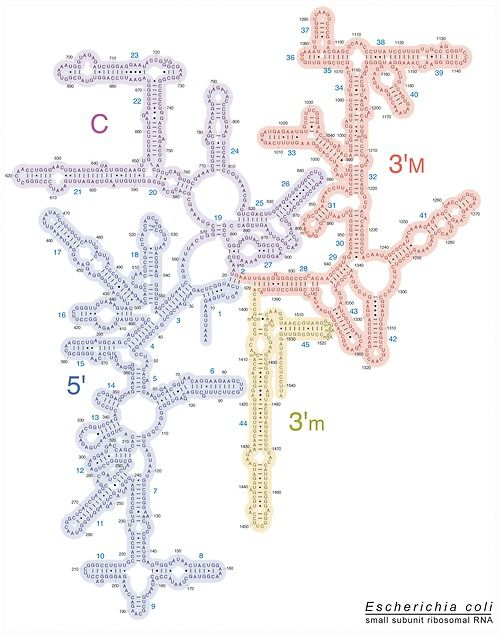
\includegraphics[width = 0.45\linewidth]{pic/16.jpg}
    \end{center}
    
\end{frame}

\begin{frame}[fragile] \frametitle{Formal Grammars and Languages}
        \begin{itemize}
        \item $G = (\Sigma, N, R, s)$ --- context-free grammar (CFG) in Chomsky normal form
          \begin{itemize}
            \item $a \rightarrow b c$, where $a, b, c \in N$
            \item $a \rightarrow A$, where $a \in N, A \in \Sigma$
            \item $s \rightarrow \varepsilon$, where $\varepsilon$ is an empty string
          \end{itemize}
        \item $L_G (s) = \{ \omega \mid s \Rightarrow^* \omega \}$, where $\omega \in \Sigma^*$
        \item Parsing --- does $\omega$ belong to $ L_G (s)$?

        \end{itemize}
\end{frame}

\begin{frame}[fragile] \frametitle{CFG-based Approach}

    \begin{itemize}
        \item RNA sequences are treated as strings over $\Sigma = \{A, G, C, U\}$
        $$
        \texttt{CACGACUGUACUUAGUCUC\dots CUGGAUCACCUCCUU}
        $$
        \item CFG describes RNA secondary structure features
    \end{itemize}
        \begin{figure}[t]
            %\subfloat
        \end{figure}

        \vspace{-100pt}\hspace{30pt}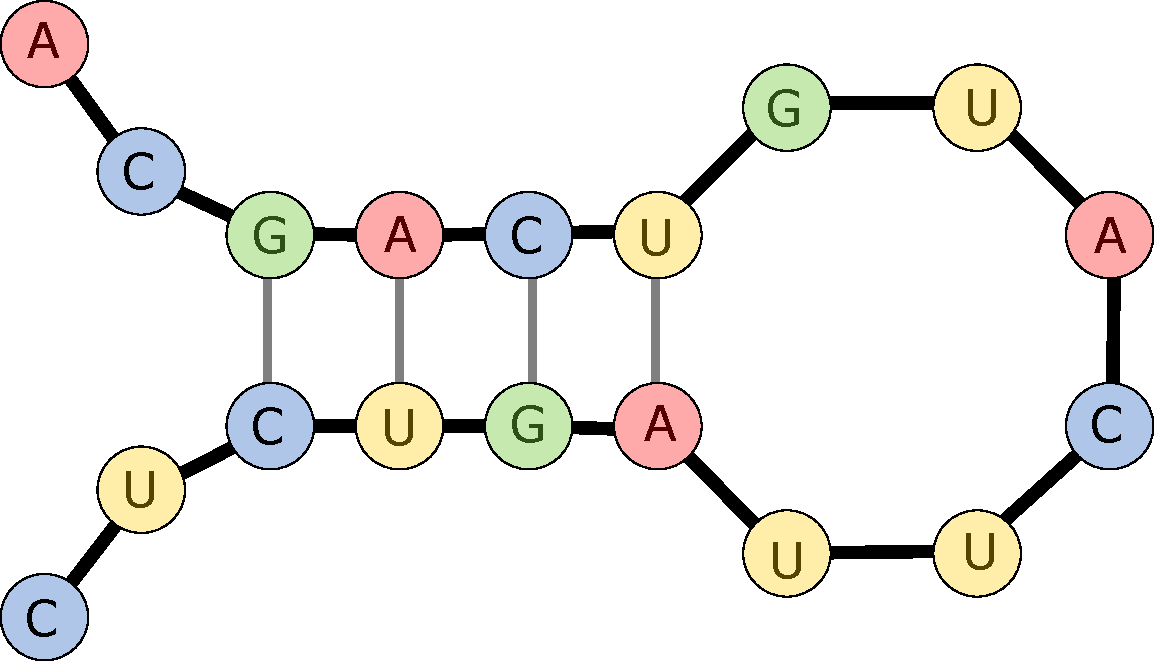
\includegraphics[width = 0.4\linewidth]{pic/16s.pdf}\par 
        \pause
        \begin{itemize}
            \item Parsing as method to find all substrings with specific secondary structure features
            \item \textbf{String-searching problem:} for input string of length $n = 2^p - 1$ find all substrings of length \textit{m} which belong to $L_G(s)$
        \end{itemize}

\end{frame}




\begin{frame}[fragile] \frametitle{Problems}

    \begin{itemize}
        \item Long sequences
        \item Large amount of data
        \item Complex models
        \hspace{20pt}\smash{\raisebox{.5\dimexpr2\baselineskip+3\itemsep+2\parskip}{$\left.\rule{0pt}{.4\dimexpr4\baselineskip+3\itemsep+3\parskip}\right\}\text{computational complexity}$}}
    \end{itemize} 
    $\implies$ development of efficient parsing algorithms

\end{frame}



\begin{frame}[fragile] \frametitle{Tabular Parsing Algorithms}

\begin{itemize}
    \item Input:
    \begin{itemize}
        \item Grammar $G = (\Sigma, N, R, s)$ in Chomsky normal form
        \item String $\omega = \omega_{1}\omega_{2} \dots \omega_{n}$, $\omega_i \in \Sigma$
    \end{itemize}
    \item Parsing table $T$:
        \begin{itemize}
            \item $T_{i, j} =  \{ a \mid a \in N, \omega_{i + 1} \dots \omega_{j} \in L_{G}(a)\} \quad \forall i < j$
            \item $\omega \in L_{G}(s) \iff s \in T_{0, n}$
        \end{itemize}
    \pause
    \item Process of filling:
        \begin{itemize}
            \item $T_{i - 1, i} = \{ a \mid a \rightarrow \omega_{i} \in R\}$
            \vspace{5pt}
            \item $T_{i, j} = f(P_{i, j})$, where $P_{i, j} = \bigcup\limits_{k = i + 1}^{j - 1} T_{i,k} \times T_{k, j}$ \\ 
            \hspace{85pt} $f(P_{i, j}) = \{a \mid \exists a \rightarrow bc \in R : (b, c) \in P_{i, j}\}$
        \end{itemize}
    \end{itemize}
    \onslide<3>{\tikz[overlay,remember picture]{\draw[draw=red,thick,double,fill opacity=0.1] ($(5.6,0.96)$) rectangle ($ (8.2,2.1)$);}}
\end{frame}

\begin{frame}[fragile] \frametitle{To Valiant's Parsing Algorithm}

    \begin{center}
        
    CYK: $\mathcal{O}(|G|n^3)$  \\
    \emph{Younger, D. H.} "Context-free language processing in time $n^3$" 1966
    
    $\Downarrow$ 
    
    Reduction to matrix multiplication 
    
    $\Downarrow $
    
    Reduction to Boolean matrix multiplication 
    
    $\Downarrow$ 
    
    Valiant: $\mathcal{O}(|G|BMM(n)log(n))$ \\
    \emph{Valiant, L. G.} "General context-free recognition in less than cubic time" 1975
    
    \end{center}

\onslide<2>{\tikz[overlay,remember picture]{\draw[draw=red,thick,double,fill opacity=0.2] ($(0.2,0.65)$) rectangle ($ (12,2.25)$);}}

\end{frame}


\begin{frame}[fragile] \frametitle{Valiant's Algorithm}

    \begin{itemize}
    \item (+):
    \begin{itemize}
        \item Utilization of parallel techniques and highly-efficient libraries
        \item Generalization to more powerful classes of formal grammars: conjunctive and Boolean
    \end{itemize}
    \item (---):
    \begin{itemize}
      \item Not suitable for string-searching problem \\
      It is necessary to calculate at least 2 triangle submatrices of size $\frac{n}{2}$ 
    \end{itemize}
    \end{itemize}

    \begin{overprint}
    \onslide<1>
    \[
    \underbrace{\centering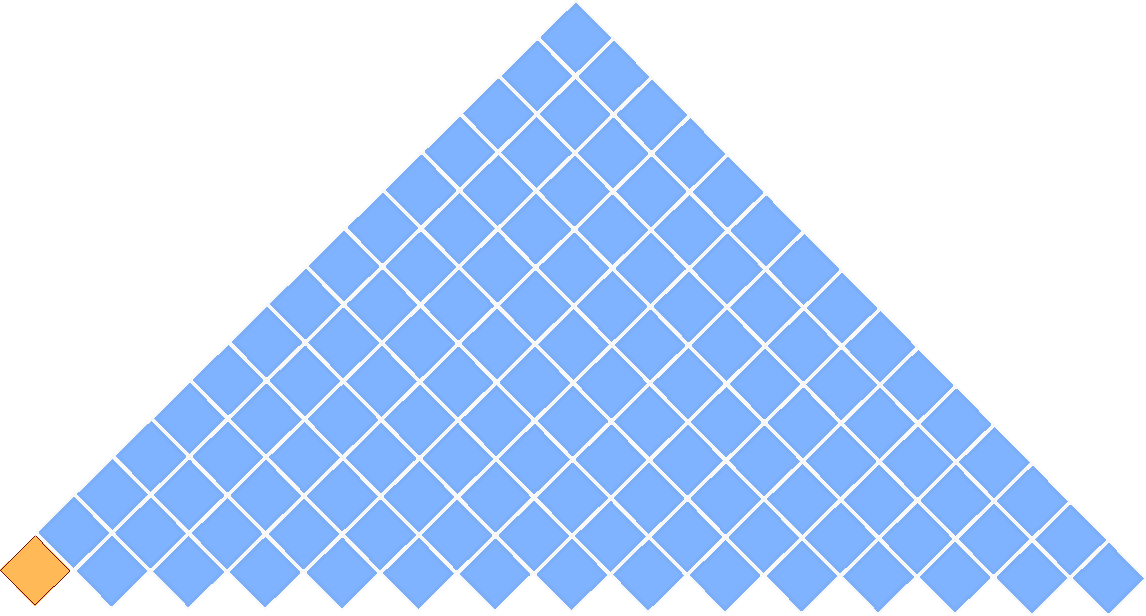
\includegraphics[width = 0.5\linewidth]{pic/vv001.pdf}}_{\text{$\omega = \omega_{1}\omega_{2} \dots \omega_{15} $}}
    \]
    \onslide<2>
    \[
    \underbrace{\centering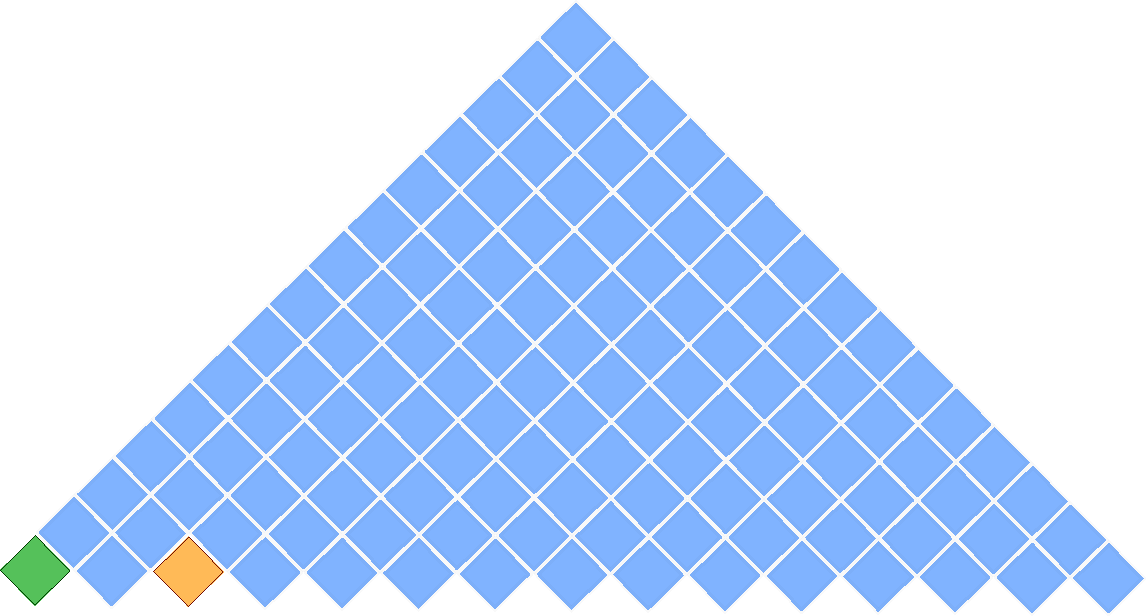
\includegraphics[width = 0.5\linewidth]{pic/vv002.pdf}}_{\text{$\omega = \omega_{1}\omega_{2} \dots \omega_{15} $}}
    \]
    \onslide<3>
    \[
    \underbrace{\centering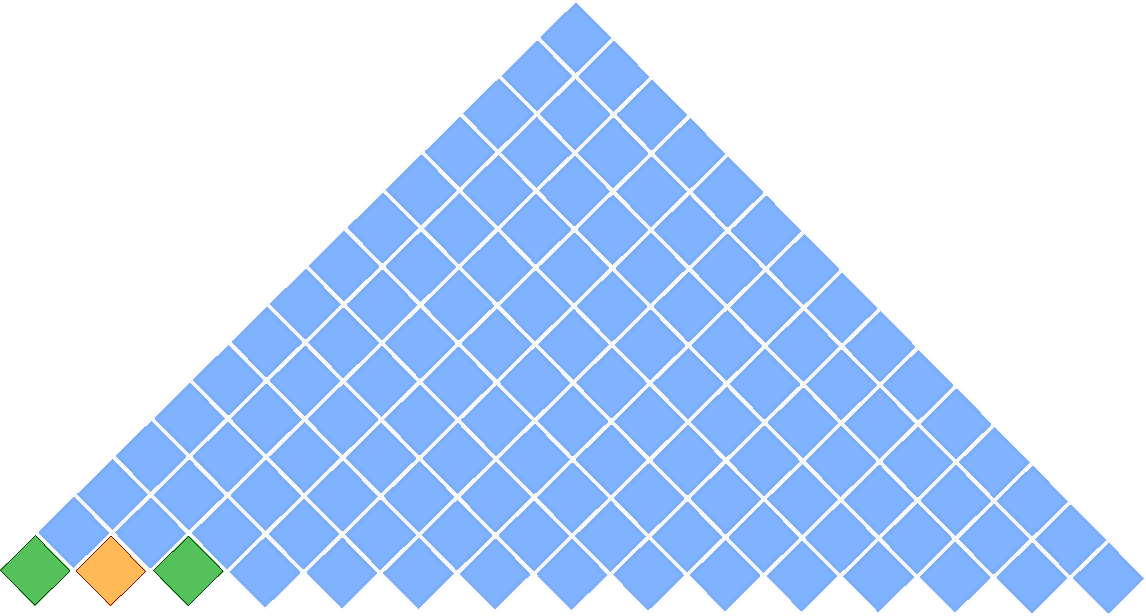
\includegraphics[width = 0.5\linewidth]{pic/vv003.pdf}}_{\text{$\omega = \omega_{1}\omega_{2} \dots \omega_{15} $}}
    \]
    \onslide<4>
    \[
    \underbrace{\centering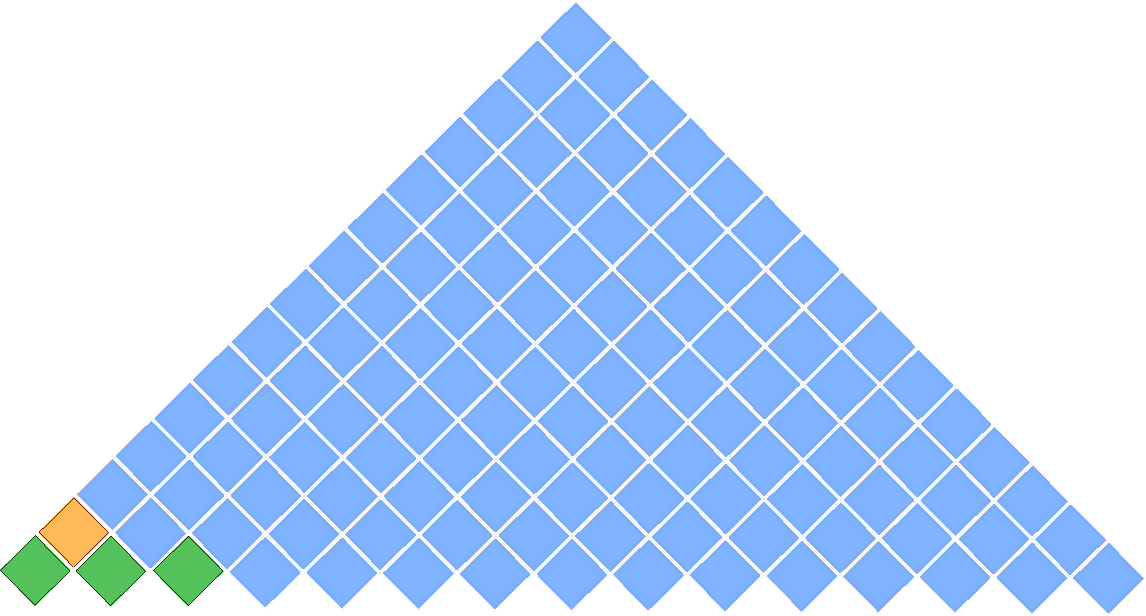
\includegraphics[width = 0.5\linewidth]{pic/vv004.pdf}}_{\text{$\omega = \omega_{1}\omega_{2} \dots \omega_{15} $}}
    \]
    \onslide<5>
    \[
    \underbrace{\centering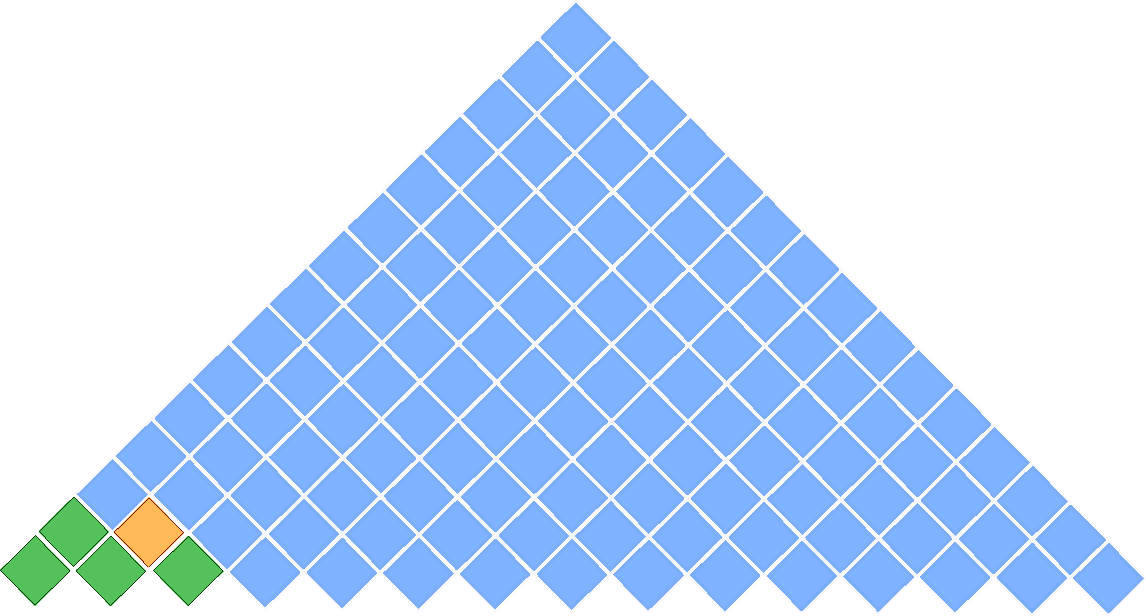
\includegraphics[width = 0.5\linewidth]{pic/vv005.pdf}}_{\text{$\omega = \omega_{1}\omega_{2} \dots \omega_{15} $}}
    \]
    \onslide<6>
    \[
    \underbrace{\centering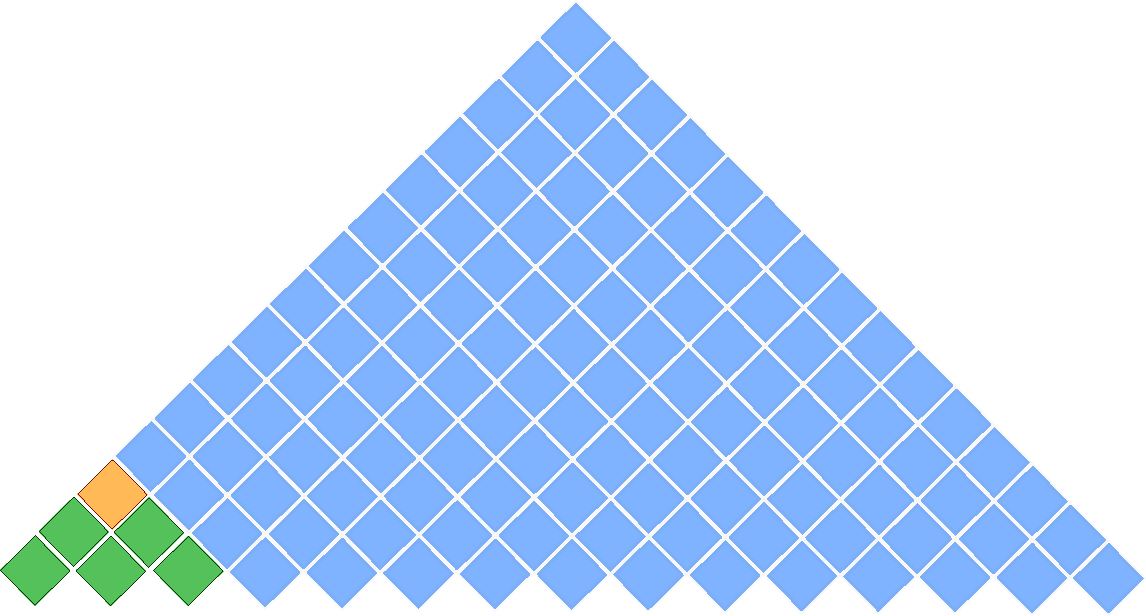
\includegraphics[width = 0.5\linewidth]{pic/vv006.pdf}}_{\text{$\omega = \omega_{1}\omega_{2} \dots \omega_{15} $}}
    \]
    \onslide<7>
    \[
    \underbrace{\centering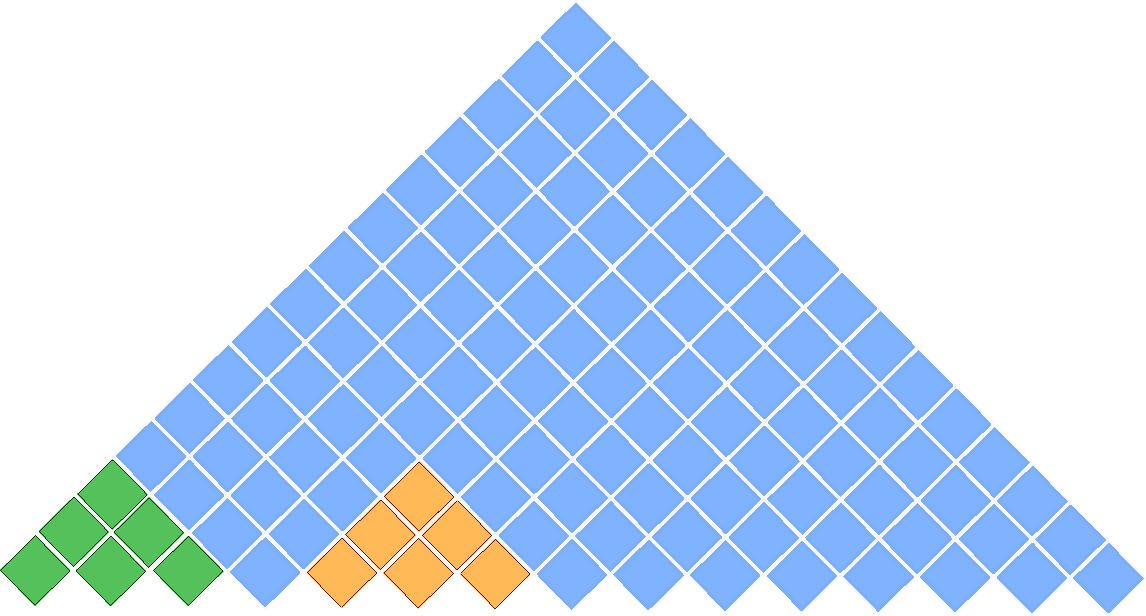
\includegraphics[width = 0.5\linewidth]{pic/vv008.pdf}}_{\text{$\omega = \omega_{1}\omega_{2} \dots \omega_{15} $}}
    \]
    \onslide<8>
    \[
    \underbrace{\centering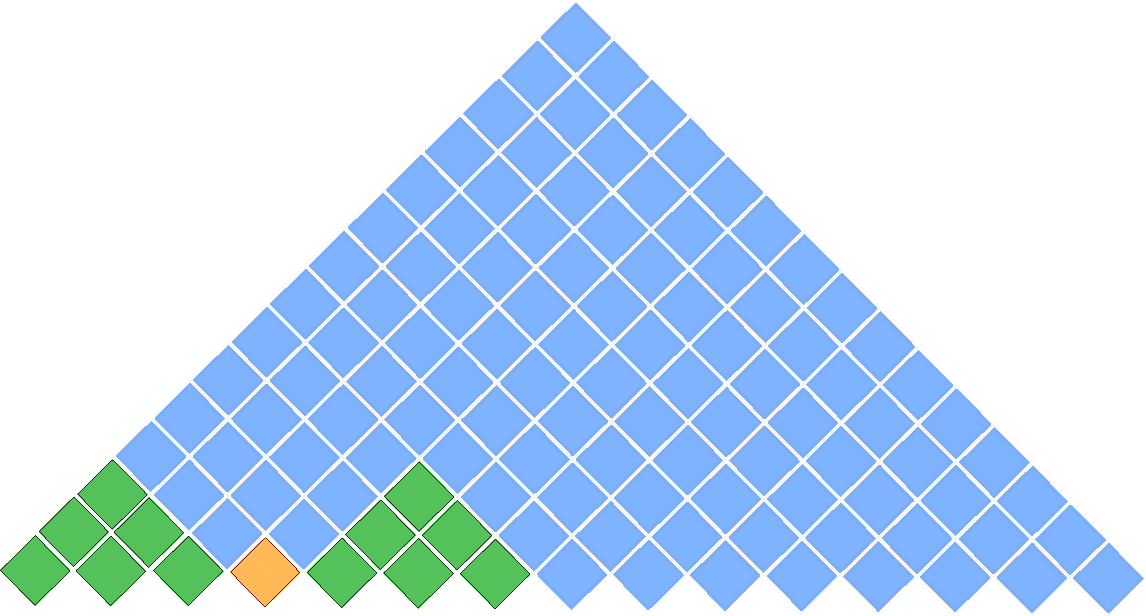
\includegraphics[width = 0.5\linewidth]{pic/vv009.pdf}}_{\text{$\omega = \omega_{1}\omega_{2} \dots \omega_{15} $}}
    \]
    \onslide<9>
    \[
    \underbrace{\centering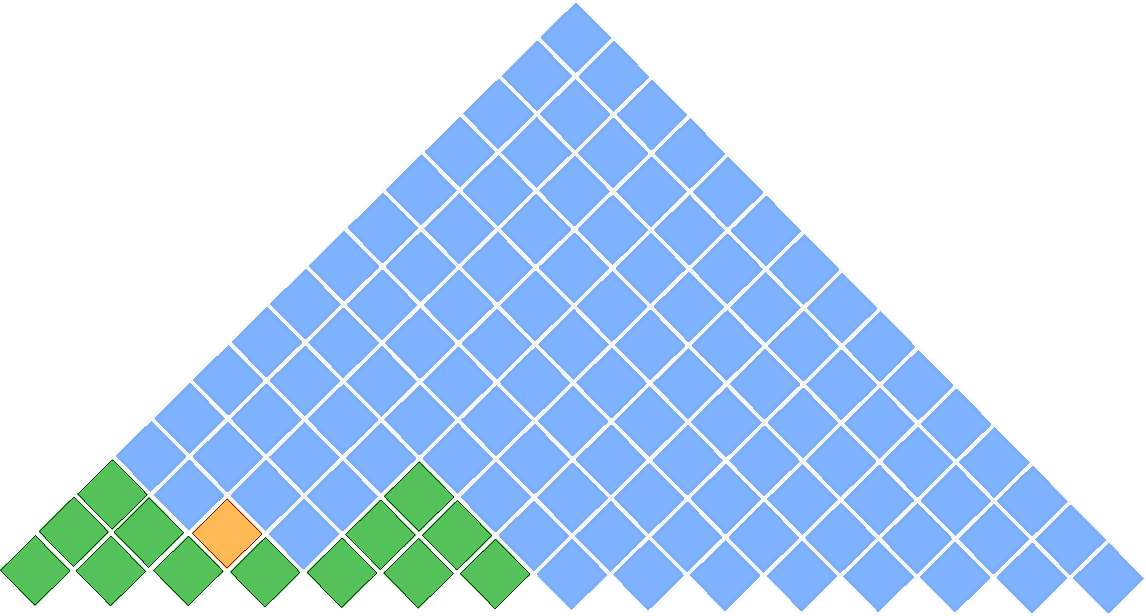
\includegraphics[width = 0.5\linewidth]{pic/vv010.pdf}}_{\text{$\omega = \omega_{1}\omega_{2} \dots \omega_{15} $}}
    \]
    \onslide<10>
    \[
    \underbrace{\centering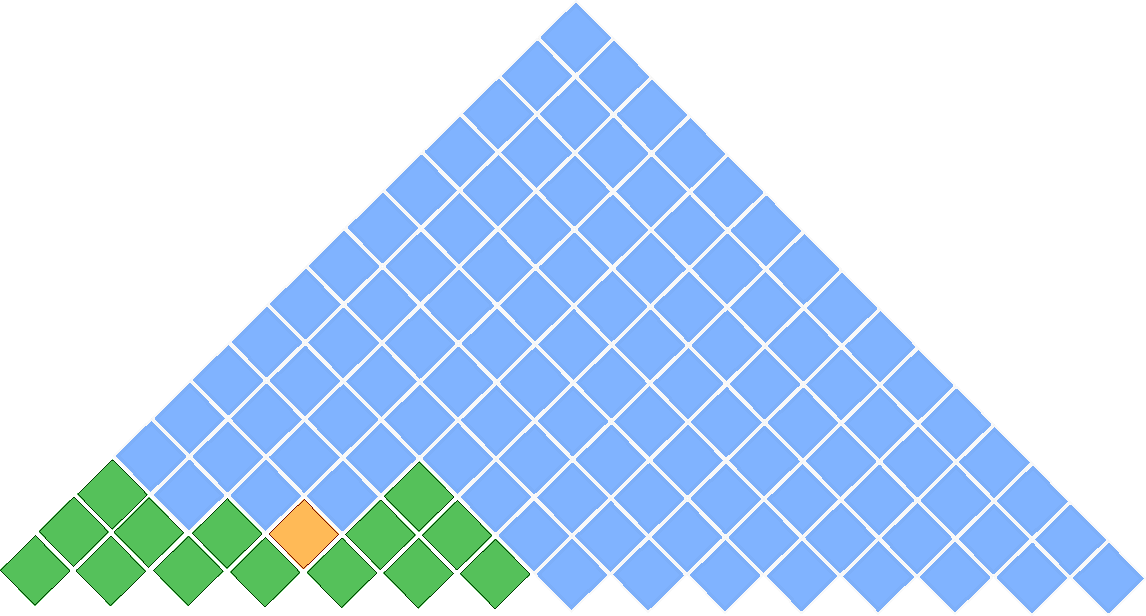
\includegraphics[width = 0.5\linewidth]{pic/vv011.pdf}}_{\text{$\omega = \omega_{1}\omega_{2} \dots \omega_{15} $}}
    \]
    \onslide<11>
    \[
    \underbrace{\centering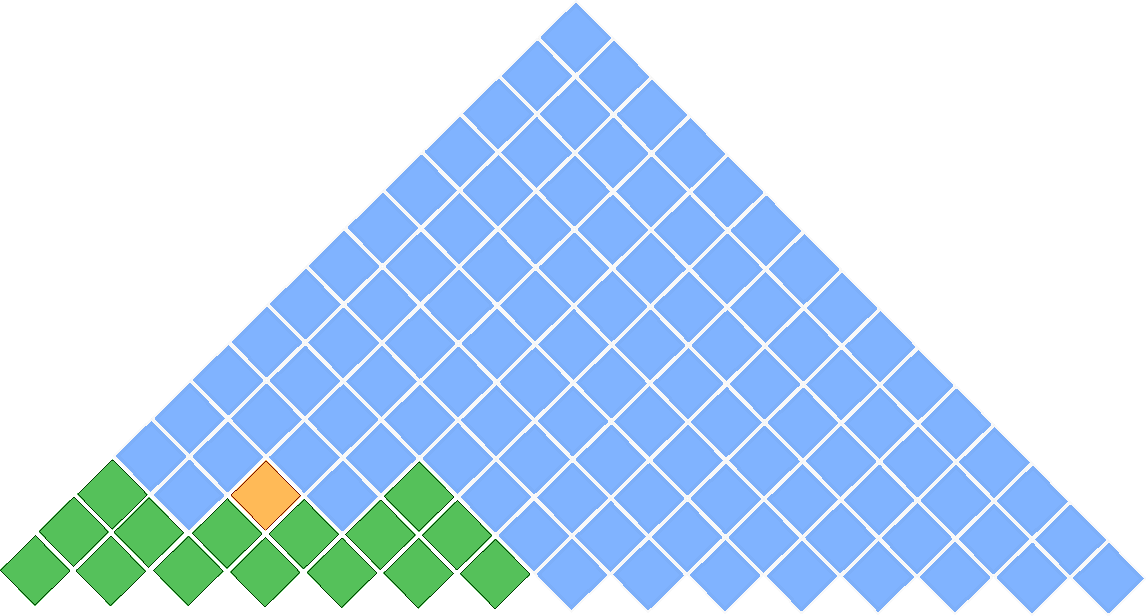
\includegraphics[width = 0.5\linewidth]{pic/vv012.pdf}}_{\text{$\omega = \omega_{1}\omega_{2} \dots \omega_{15} $}}
    \]
    \onslide<12>
    \[
    \underbrace{\centering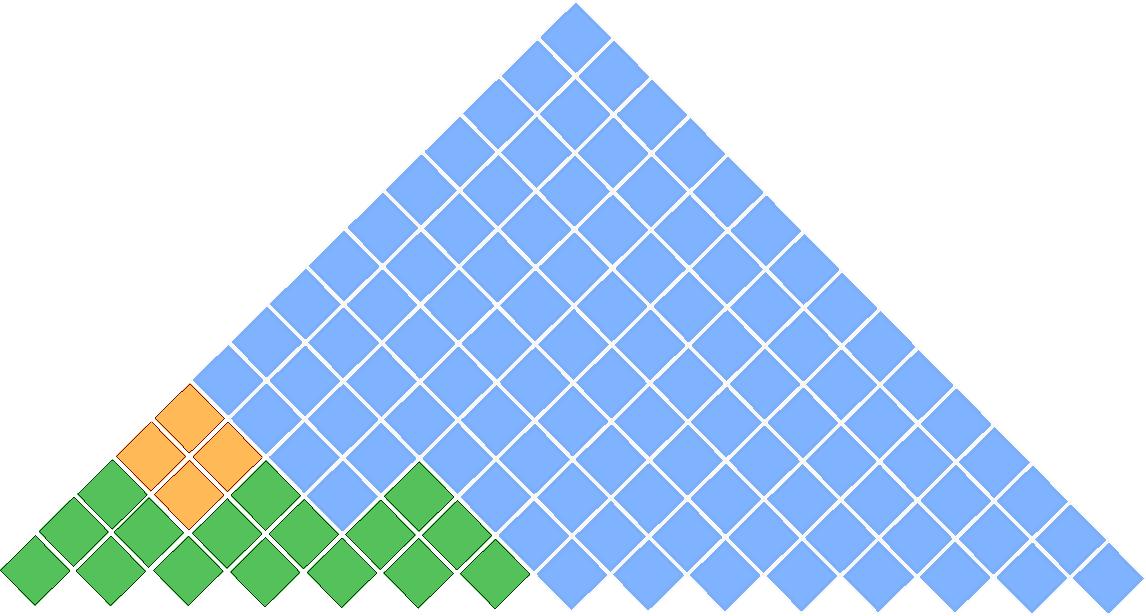
\includegraphics[width = 0.5\linewidth]{pic/vv013.pdf}}_{\text{$\omega = \omega_{1}\omega_{2} \dots \omega_{15} $}}
    \]
    \onslide<13>
    \[
    \underbrace{\centering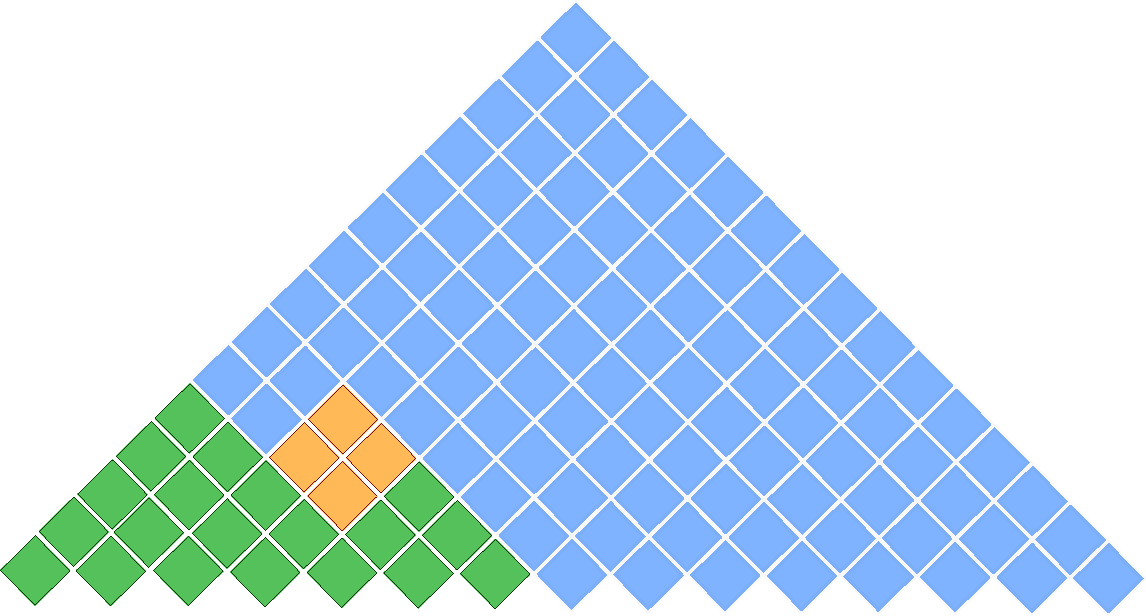
\includegraphics[width = 0.5\linewidth]{pic/vv014.pdf}}_{\text{$\omega = \omega_{1}\omega_{2} \dots \omega_{15} $}}
    \]
    \onslide<14>
    \[
    \underbrace{\centering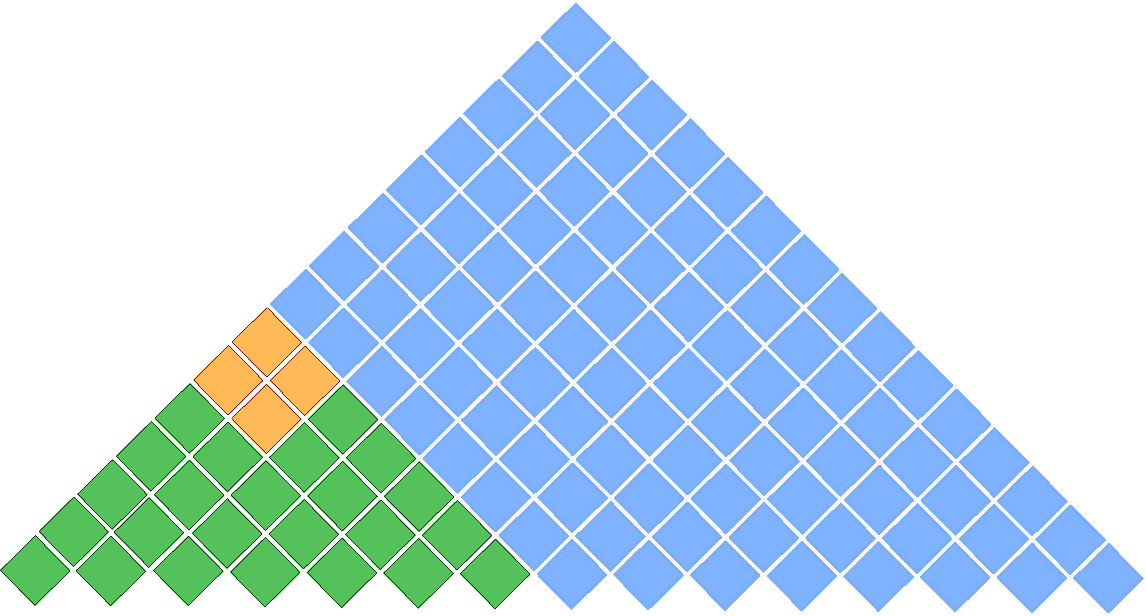
\includegraphics[width = 0.5\linewidth]{pic/vv015.pdf}}_{\text{$\omega = \omega_{1}\omega_{2} \dots \omega_{15} $}}
    \]
    \onslide<15>
    \[
    \underbrace{\centering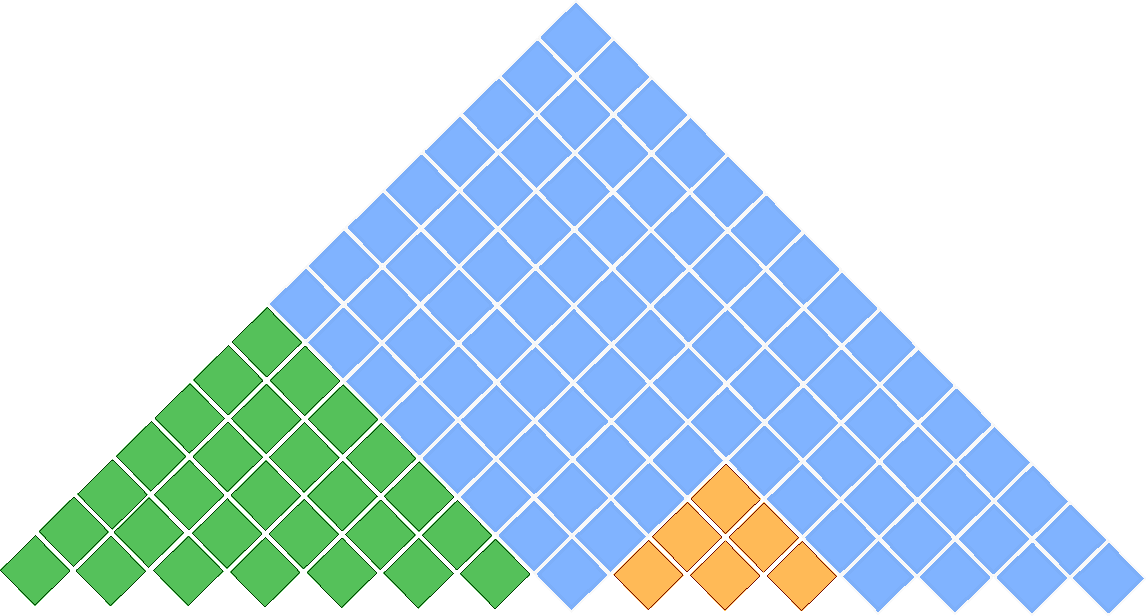
\includegraphics[width = 0.5\linewidth]{pic/vv016.pdf}}_{\text{$\omega = \omega_{1}\omega_{2} \dots \omega_{15} $}}
    \]
    \onslide<16>
    \[
    \underbrace{\centering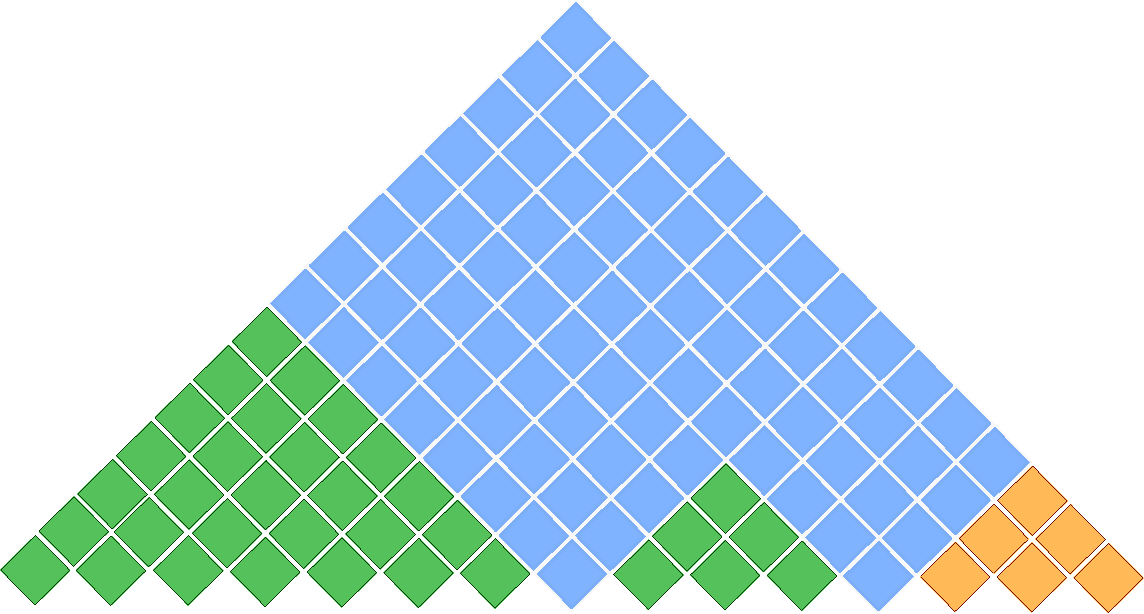
\includegraphics[width = 0.5\linewidth]{pic/vv017.pdf}}_{\text{$\omega = \omega_{1}\omega_{2} \dots \omega_{15} $}}
    \]
    \onslide<17>
    \[
    \underbrace{\centering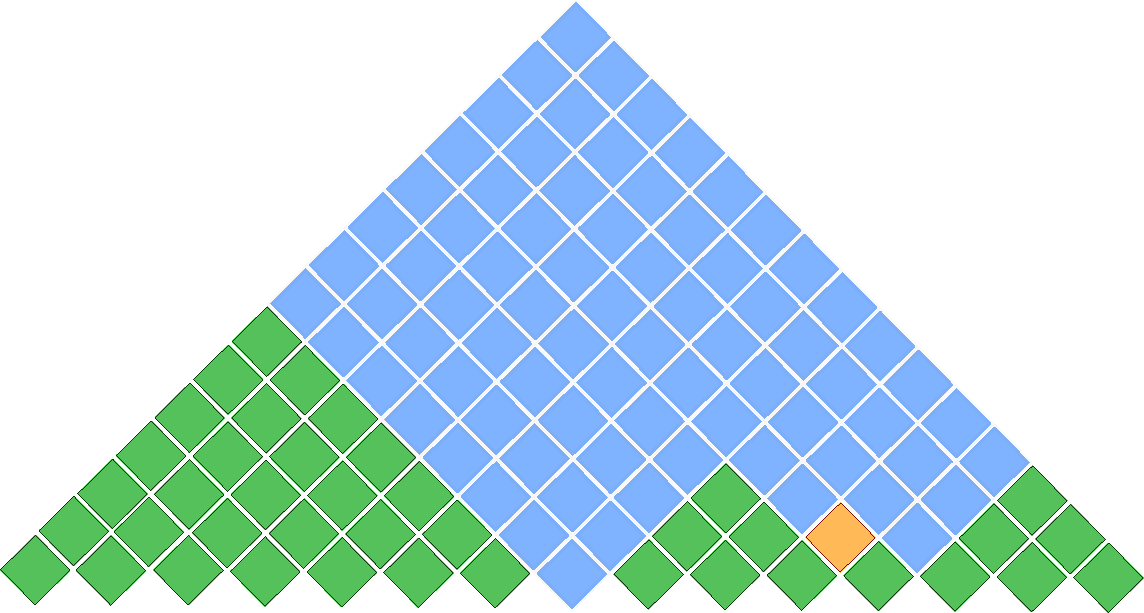
\includegraphics[width = 0.5\linewidth]{pic/vv018.pdf}}_{\text{$\omega = \omega_{1}\omega_{2} \dots \omega_{15} $}}
    \]
    \onslide<18>
    \[
    \underbrace{\centering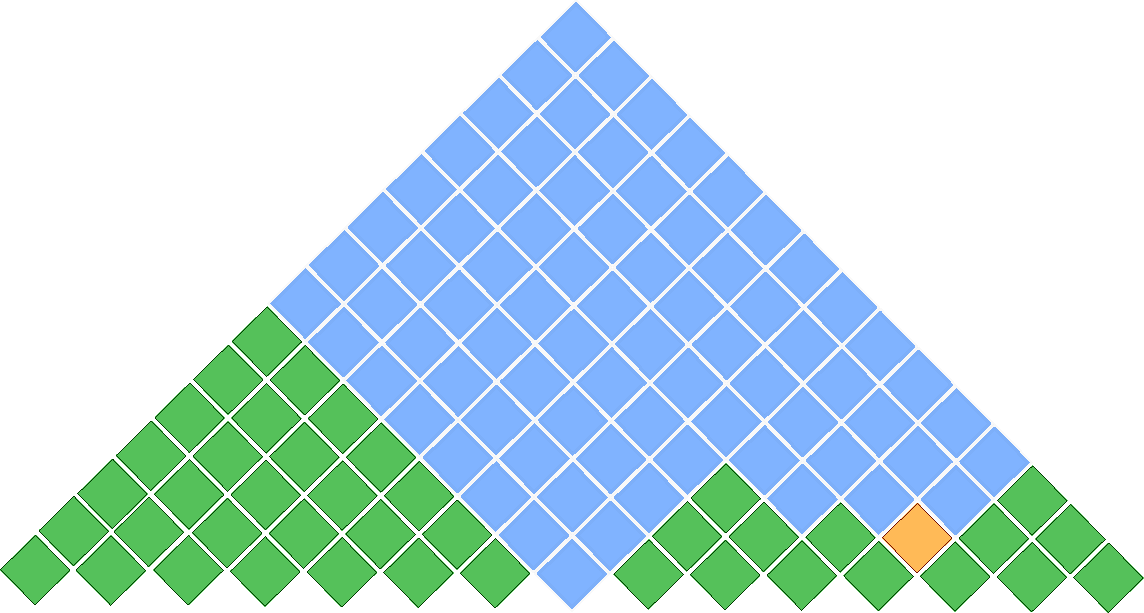
\includegraphics[width = 0.5\linewidth]{pic/vv019.pdf}}_{\text{$\omega = \omega_{1}\omega_{2} \dots \omega_{15} $}}
    \]
    \onslide<19>
    \[
    \underbrace{\centering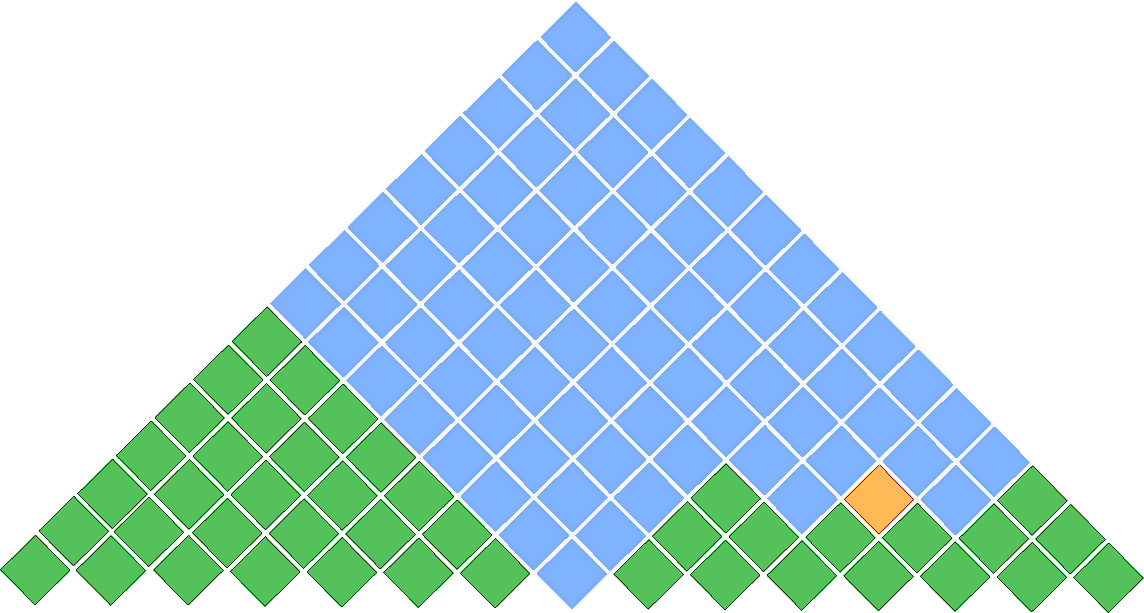
\includegraphics[width = 0.5\linewidth]{pic/vv020.pdf}}_{\text{$\omega = \omega_{1}\omega_{2} \dots \omega_{15} $}}
    \]
    \onslide<20>
    \[
    \underbrace{\centering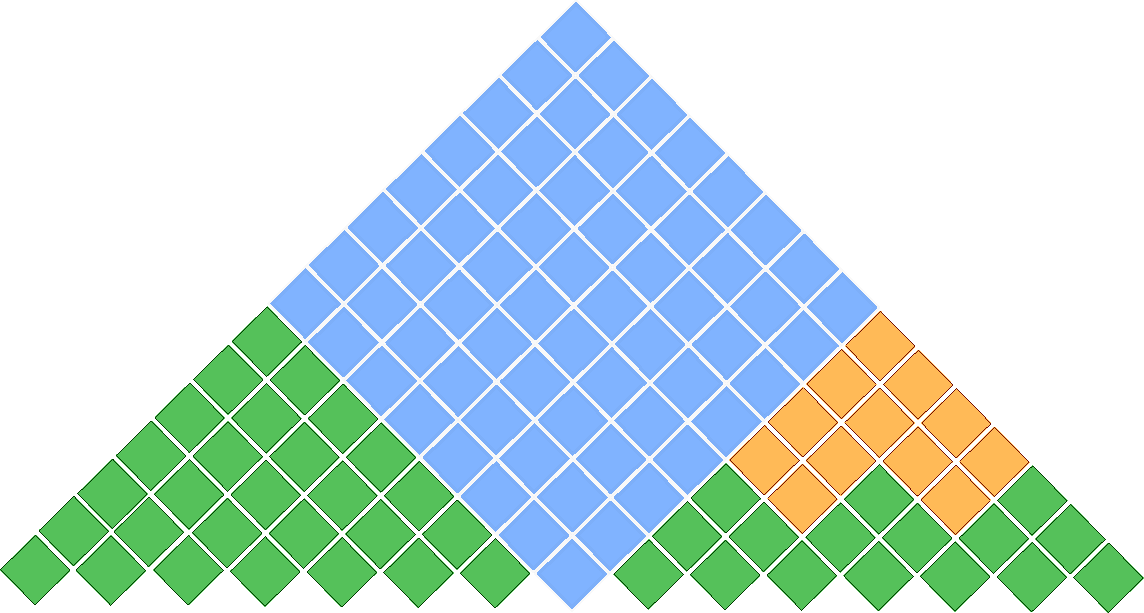
\includegraphics[width = 0.5\linewidth]{pic/vv021.pdf}}_{\text{$\omega = \omega_{1}\omega_{2} \dots \omega_{15} $}}
    \]
    \onslide<21>
    \[
    \underbrace{\centering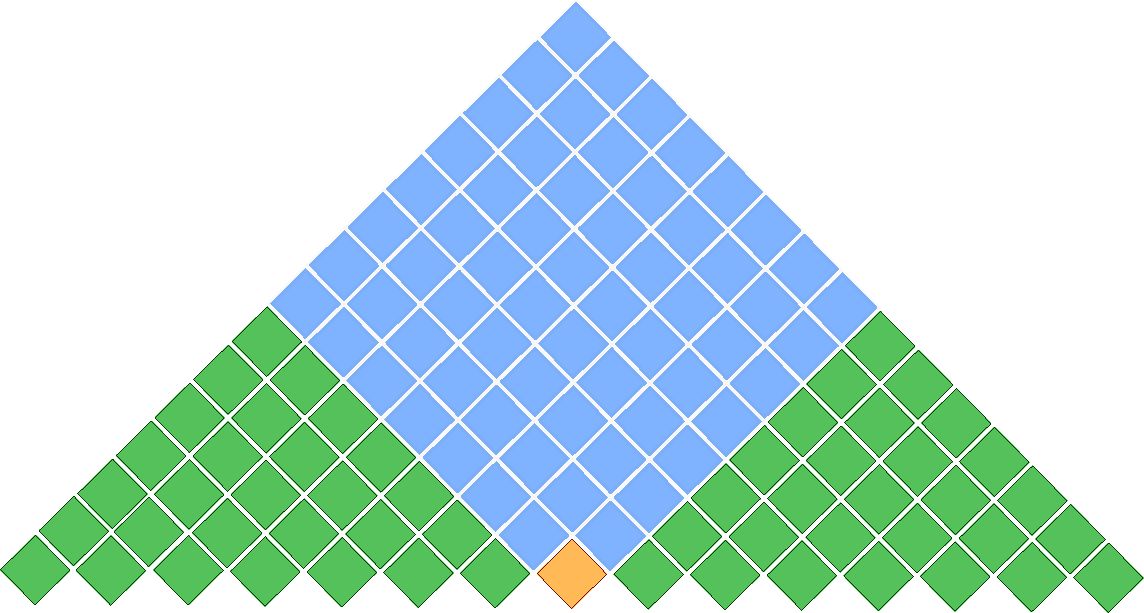
\includegraphics[width = 0.5\linewidth]{pic/vv022.pdf}}_{\text{$\omega = \omega_{1}\omega_{2} \dots \omega_{15} $}}
    \]
    \onslide<22>
    \[
    \underbrace{\centering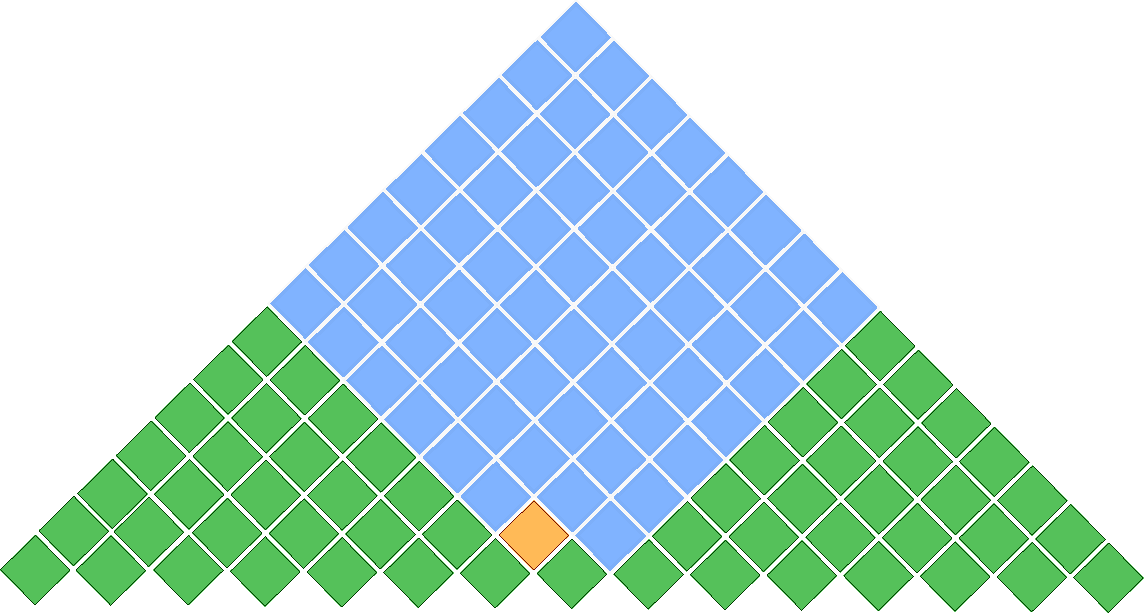
\includegraphics[width = 0.5\linewidth]{pic/vv023.pdf}}_{\text{$\omega = \omega_{1}\omega_{2} \dots \omega_{15} $}}
    \]
    \onslide<23>
    \[
    \underbrace{\centering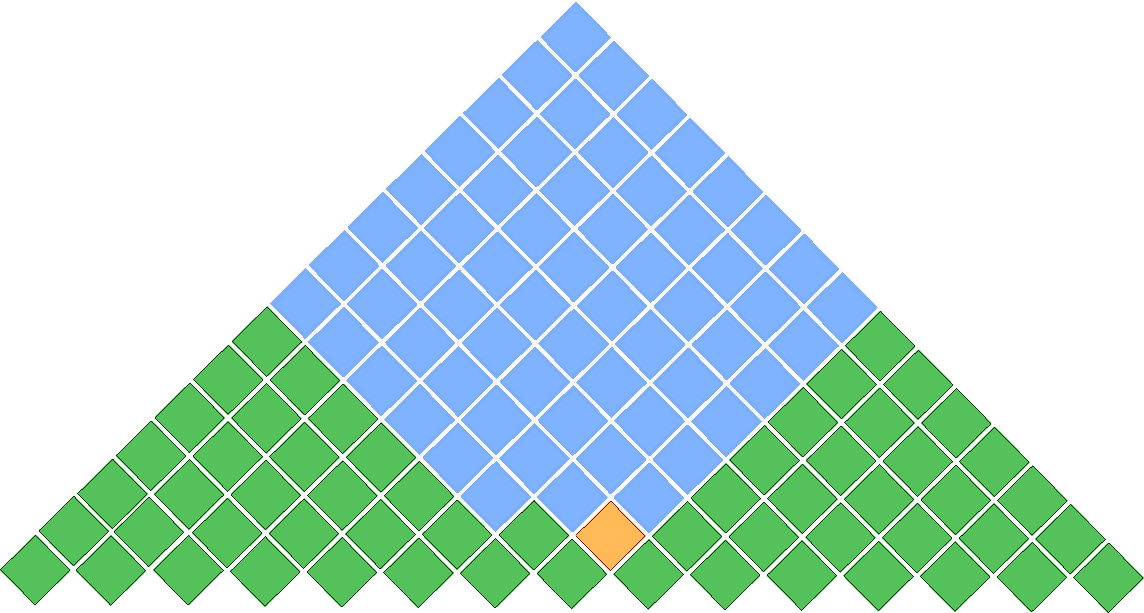
\includegraphics[width = 0.5\linewidth]{pic/vv024.pdf}}_{\text{$\omega = \omega_{1}\omega_{2} \dots \omega_{15} $}}
    \]
    \onslide<24>
    \[
    \underbrace{\centering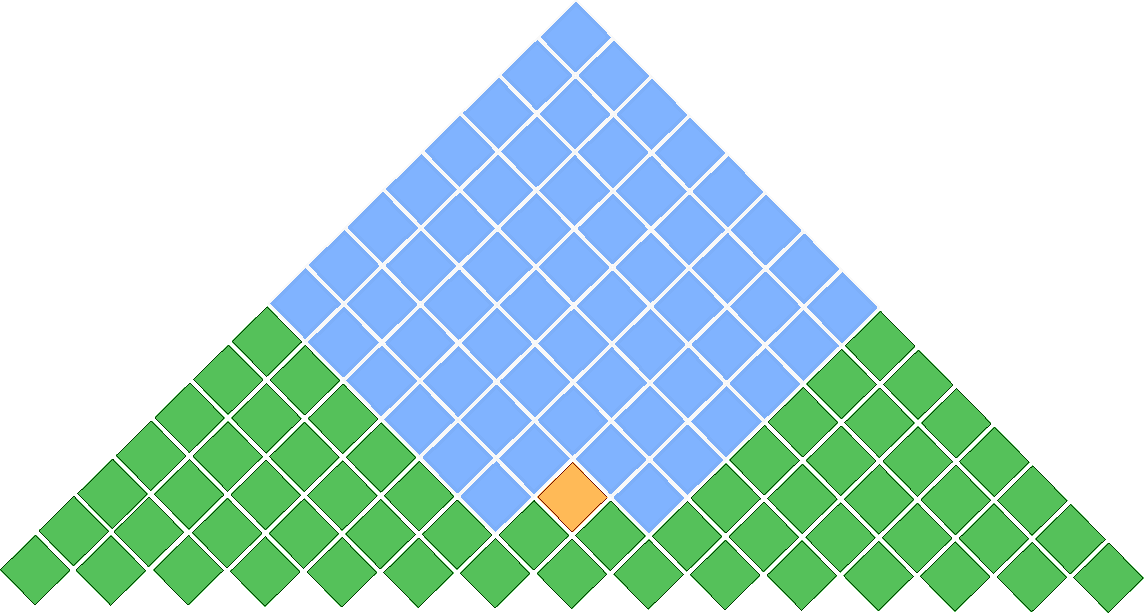
\includegraphics[width = 0.5\linewidth]{pic/vv025.pdf}}_{\text{$\omega = \omega_{1}\omega_{2} \dots \omega_{15} $}}
    \]
    \onslide<25>
    \[
    \underbrace{\centering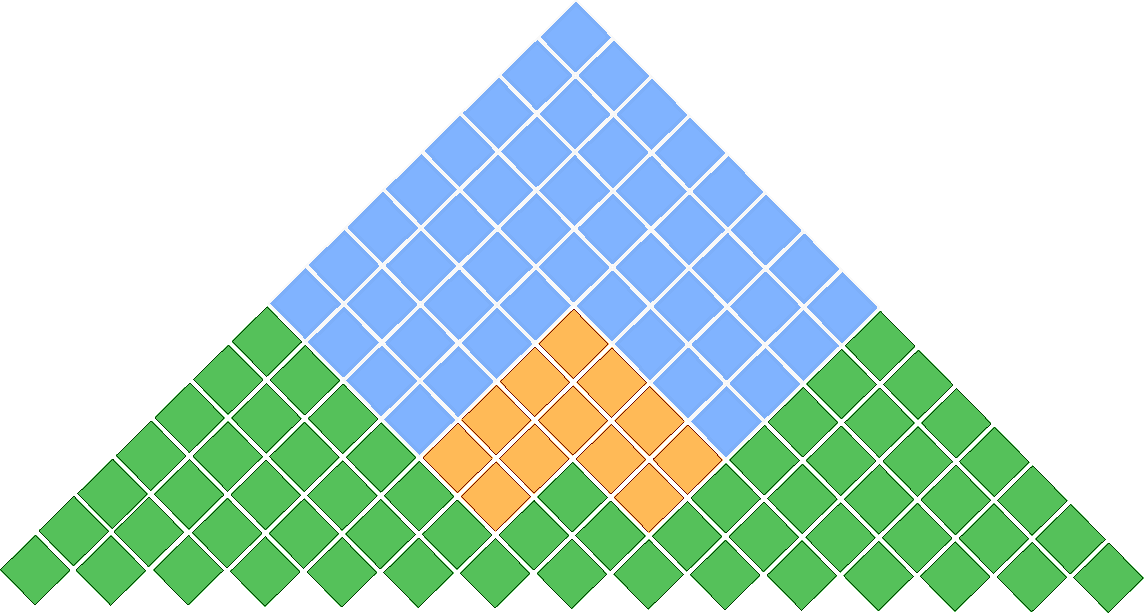
\includegraphics[width = 0.5\linewidth]{pic/vv026.pdf}}_{\text{$\omega = \omega_{1}\omega_{2} \dots \omega_{15} $}}
    \]
    \onslide<26>
    \[
    \underbrace{\centering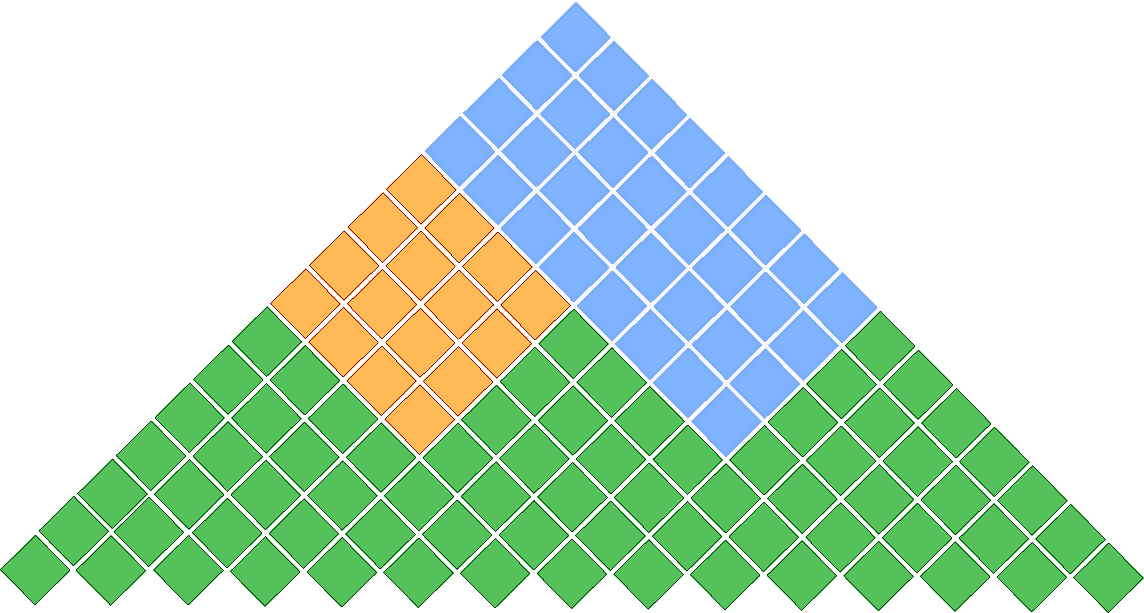
\includegraphics[width = 0.5\linewidth]{pic/vv027.pdf}}_{\text{$\omega = \omega_{1}\omega_{2} \dots \omega_{15} $}}
    \]
    \onslide<27>
    \[
    \underbrace{\centering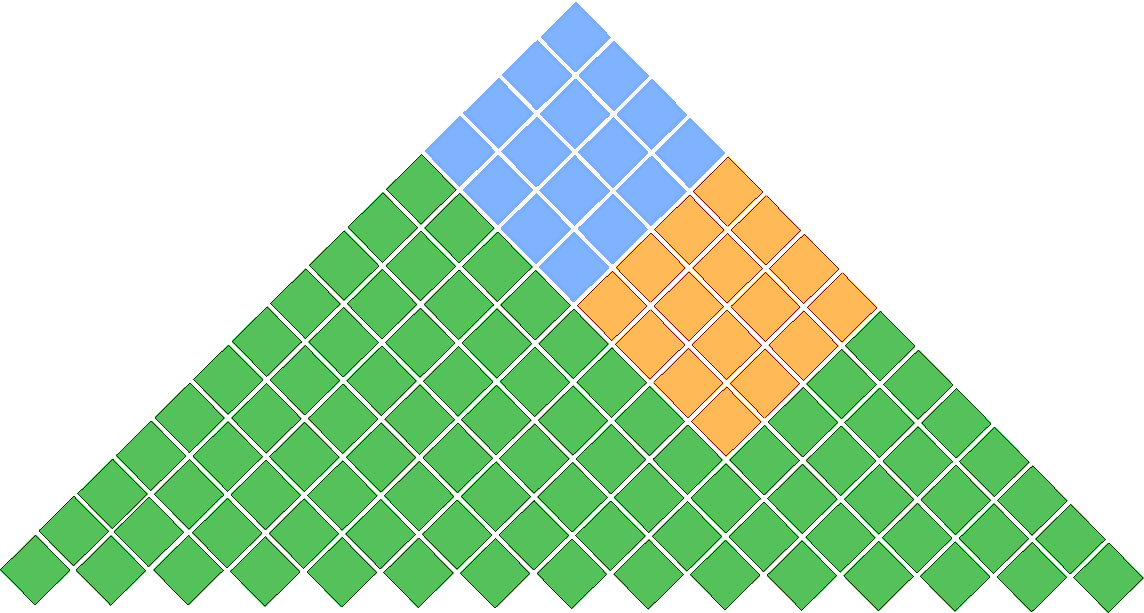
\includegraphics[width = 0.5\linewidth]{pic/vv028.pdf}}_{\text{$\omega = \omega_{1}\omega_{2} \dots \omega_{15} $}}
    \]
    \onslide<28>
    \[
    \underbrace{\centering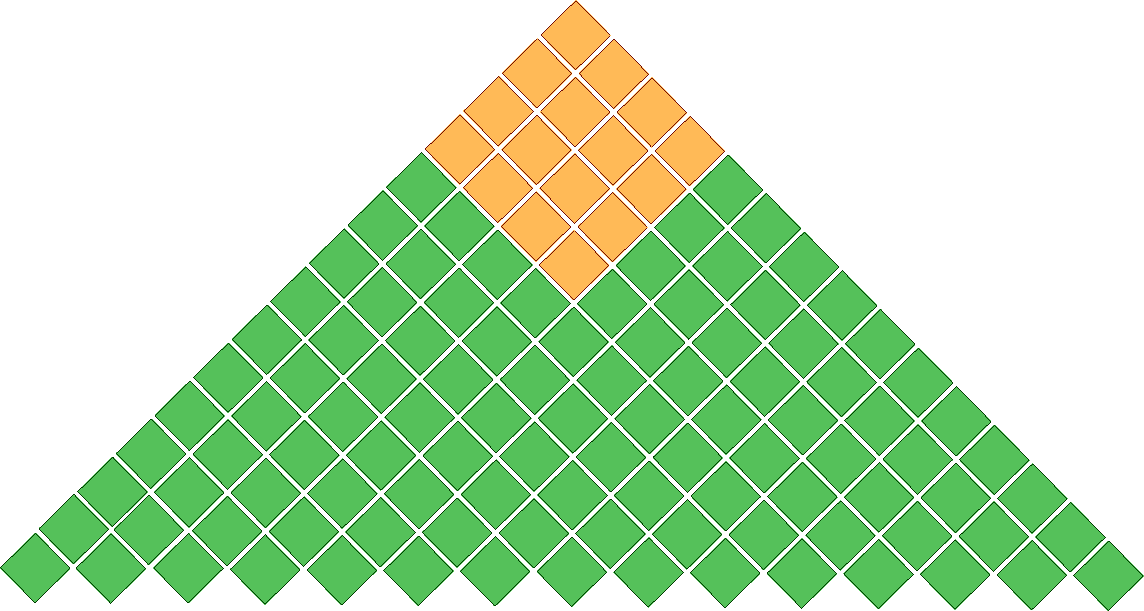
\includegraphics[width = 0.5\linewidth]{pic/vv029.pdf}}_{\text{$\omega = \omega_{1}\omega_{2} \dots \omega_{15} $}}
    \]
    \onslide<29>
    \[
    \underbrace{\centering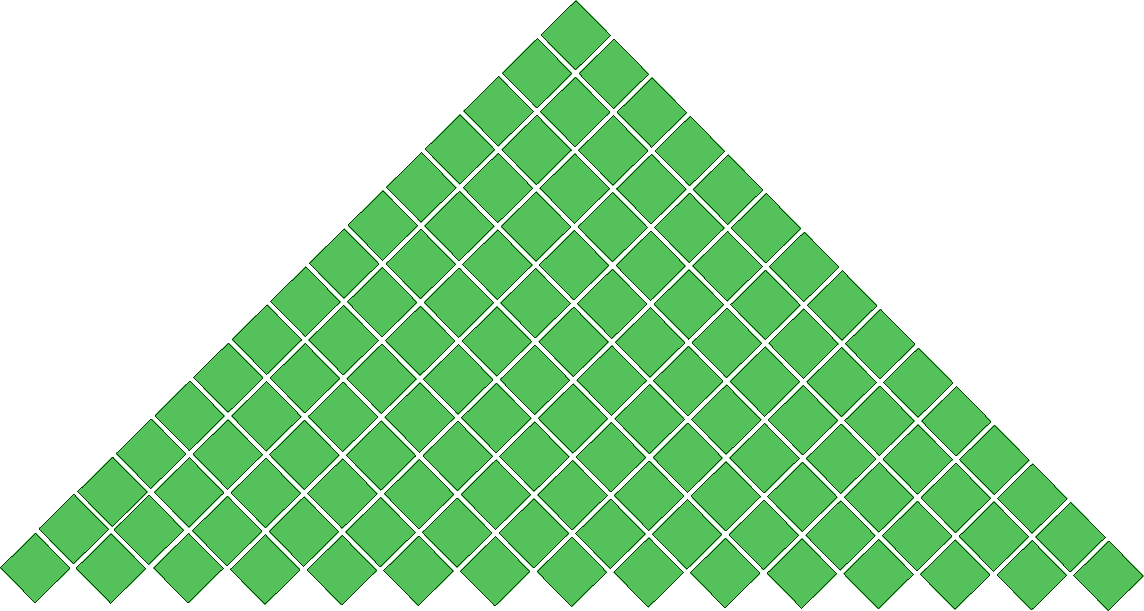
\includegraphics[width = 0.5\linewidth]{pic/vv030.pdf}}_{\text{$\omega = \omega_{1}\omega_{2} \dots \omega_{15} $}}
    \]
    \end{overprint}



\end{frame}


\begin{frame}[fragile] \frametitle{Layered Submatrices Processing (1)}

    \vspace{55pt}
    \begin{itemize}
    \item Rearranging the submatrices processing
    \item Division the parsing table into \linebreak layers of disjoint submatrices
    \end{itemize}
        
    \vspace{-130pt}\hspace{165pt}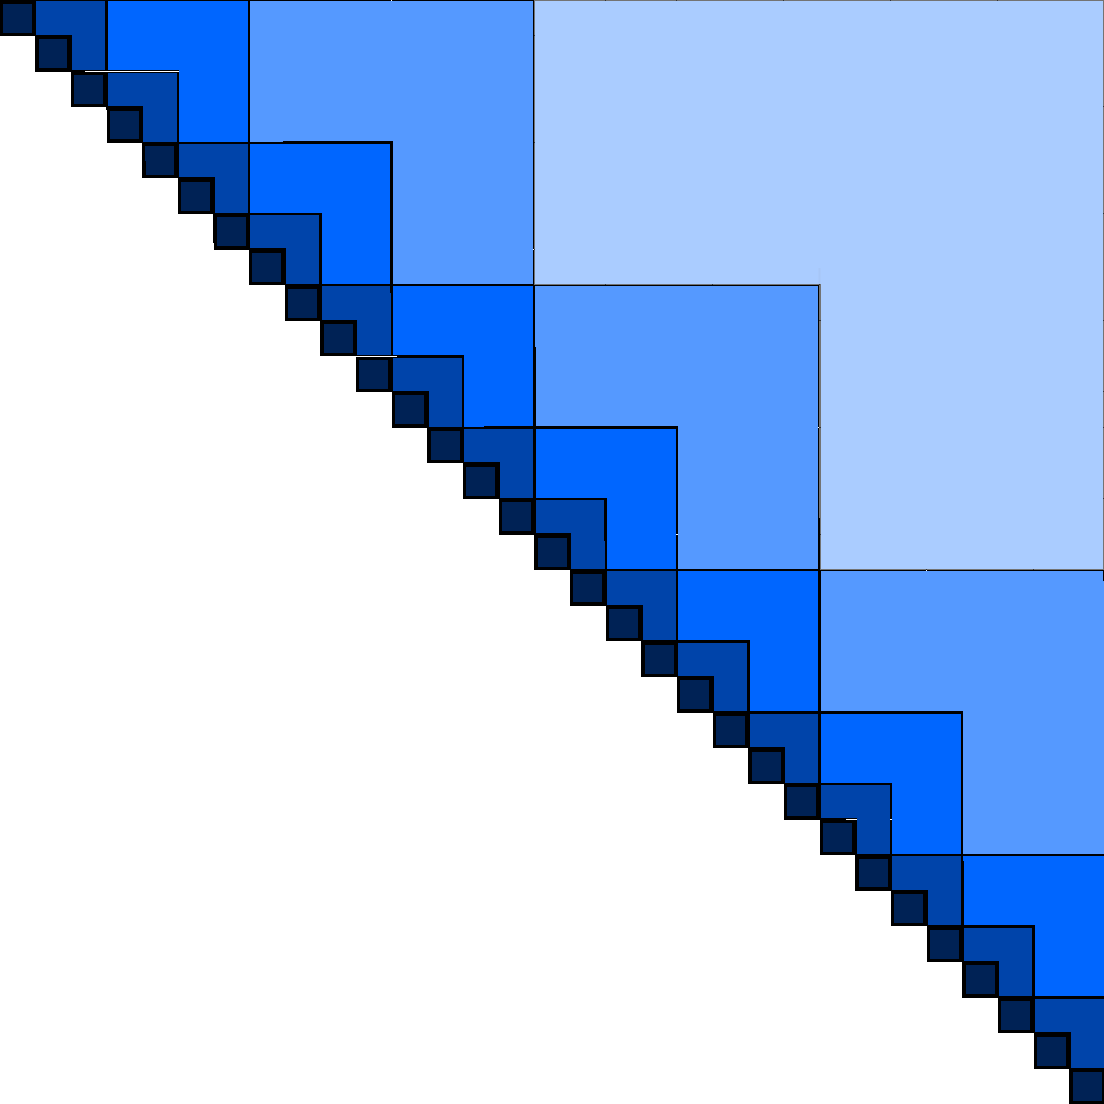
\includegraphics[width = 0.5\linewidth]{pic/layers.pdf}

    
\end{frame}

\begin{frame}[fragile] \frametitle{Layered Submatrices Processing (2)}

    \begin{itemize}
    \item Each matrix in the layer can be handled independently
    \item Increasing the lever of parallelism: 
    \begin{itemize}
        \item Matrix multiplication 
        \item Each matrix in layer
        \item Each pair of nonterminals
    \end{itemize}
    \end{itemize}

    \begin{overprint}
        \onslide<1>
        \[
        \underbrace{\centering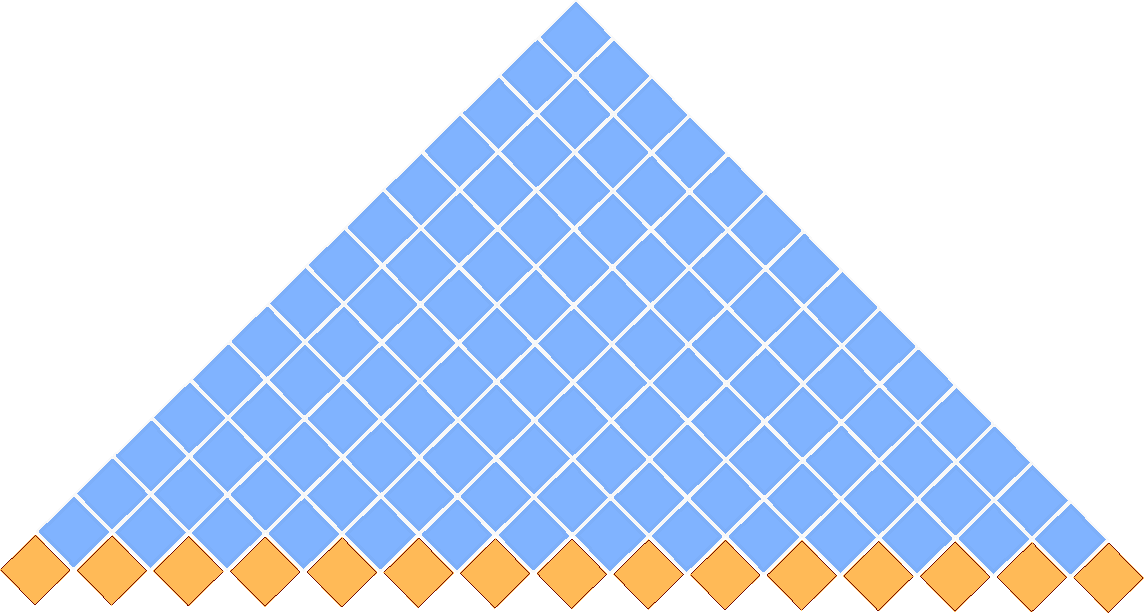
\includegraphics[width = 0.5\linewidth]{pic/mv001.pdf}}_{\text{$\omega = \omega_{1}\omega_{2} \dots \omega_{15} $}}
        \]
        \onslide<2>
        \[
        \underbrace{\centering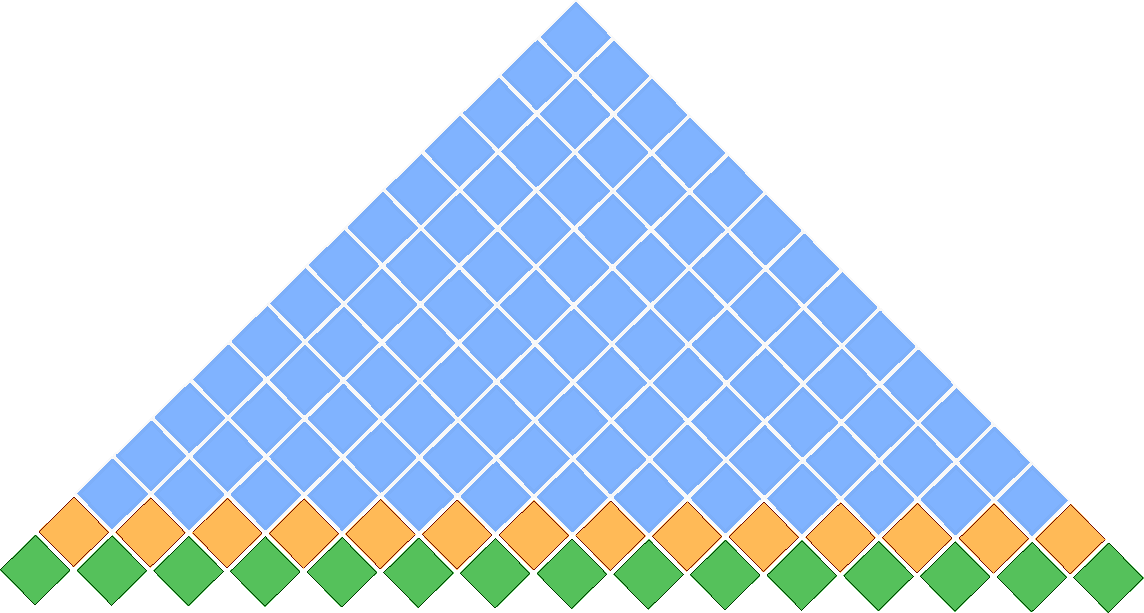
\includegraphics[width = 0.5\linewidth]{pic/mv002.pdf}}_{\text{$\omega = \omega_{1}\omega_{2} \dots \omega_{15} $}}
        \]
        \onslide<3>
        \[
        \underbrace{\centering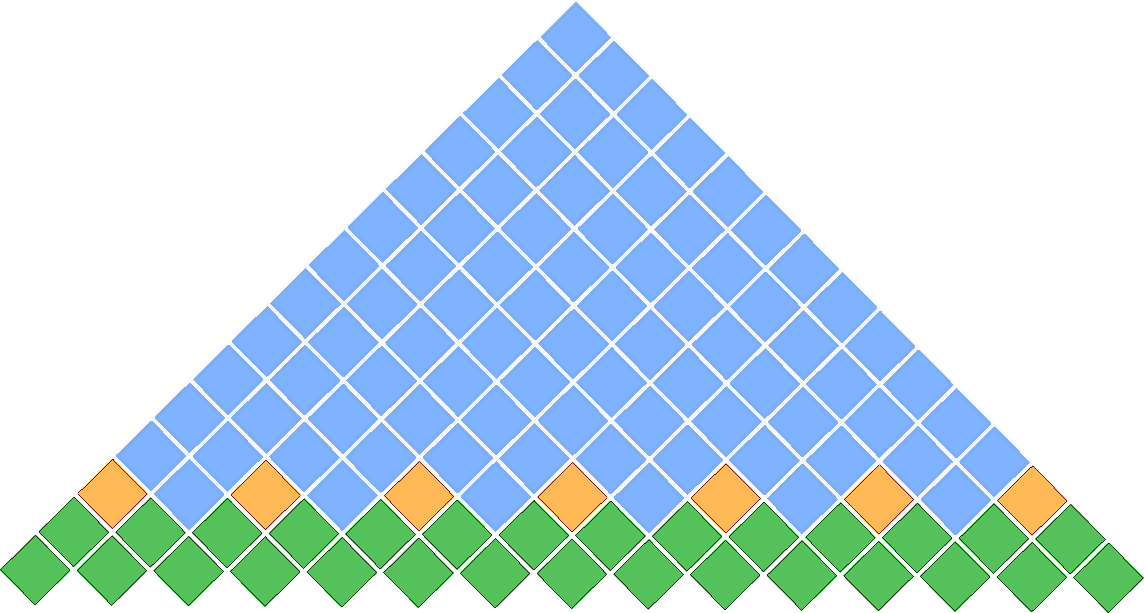
\includegraphics[width = 0.5\linewidth]{pic/mv003.pdf}}_{\text{$\omega = \omega_{1}\omega_{2} \dots \omega_{15} $}}
        \]
        \onslide<4>
        \[
        \underbrace{\centering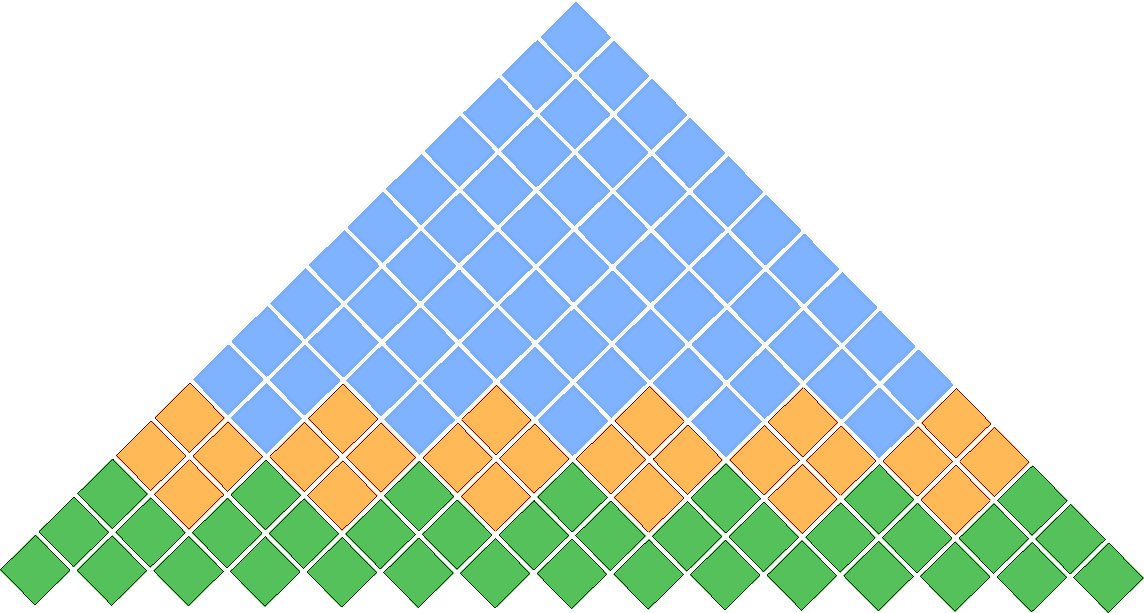
\includegraphics[width = 0.5\linewidth]{pic/mv004.pdf}}_{\text{$\omega = \omega_{1}\omega_{2} \dots \omega_{15} $}}
        \]
        \onslide<5>
        \[
        \underbrace{\centering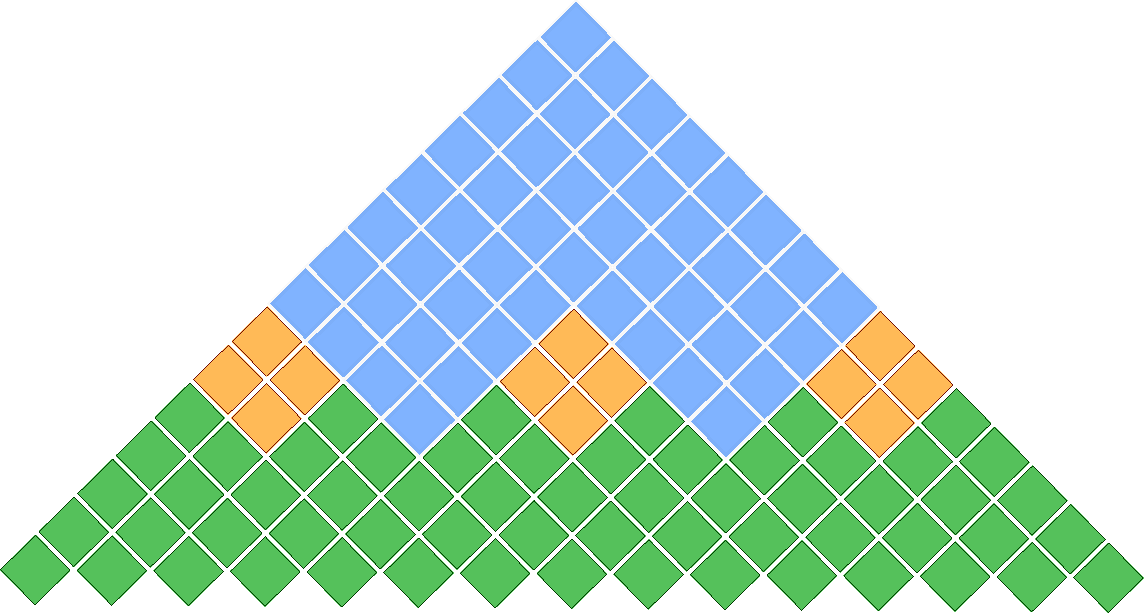
\includegraphics[width = 0.5\linewidth]{pic/mv005.pdf}}_{\text{$\omega = \omega_{1}\omega_{2} \dots \omega_{15} $}}
        \]
        \onslide<6>
        \[
        \underbrace{\centering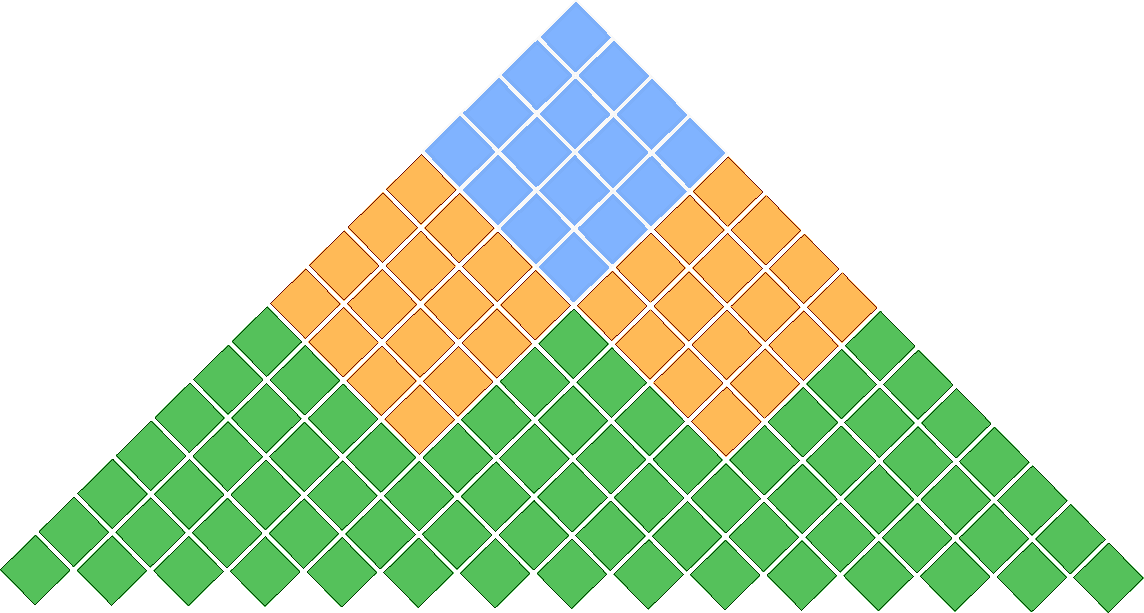
\includegraphics[width = 0.5\linewidth]{pic/mv006.pdf}}_{\text{$\omega = \omega_{1}\omega_{2} \dots \omega_{15} $}}
        \]
        \onslide<7>
        \[
        \underbrace{\centering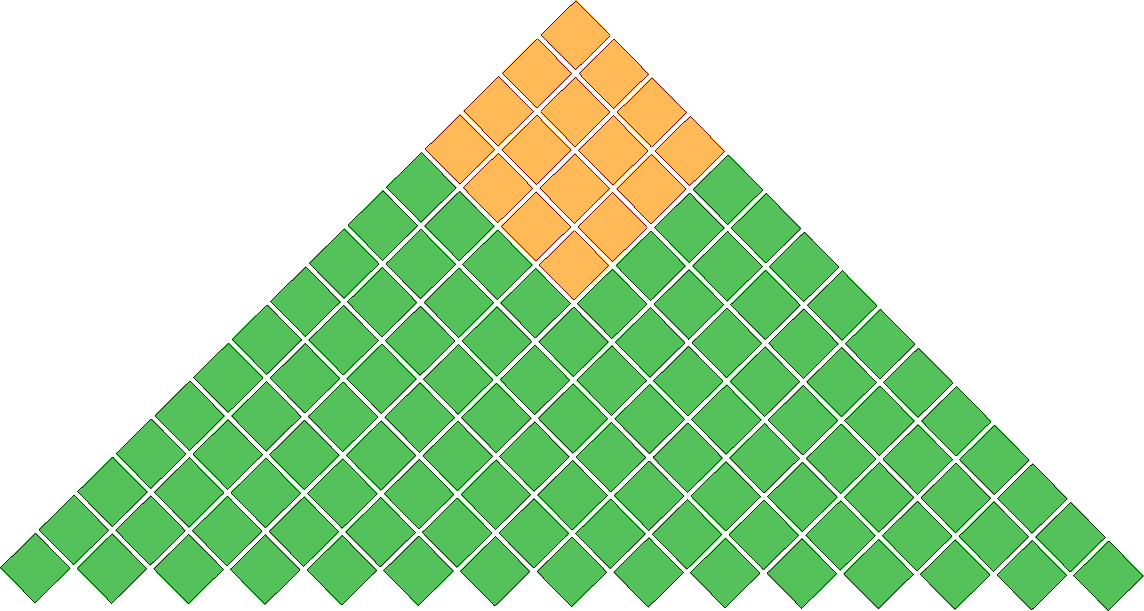
\includegraphics[width = 0.5\linewidth]{pic/mv007.pdf}}_{\text{$\omega = \omega_{1}\omega_{2} \dots \omega_{15} $}}
        \]
        \onslide<8>
         \[
        \underbrace{\centering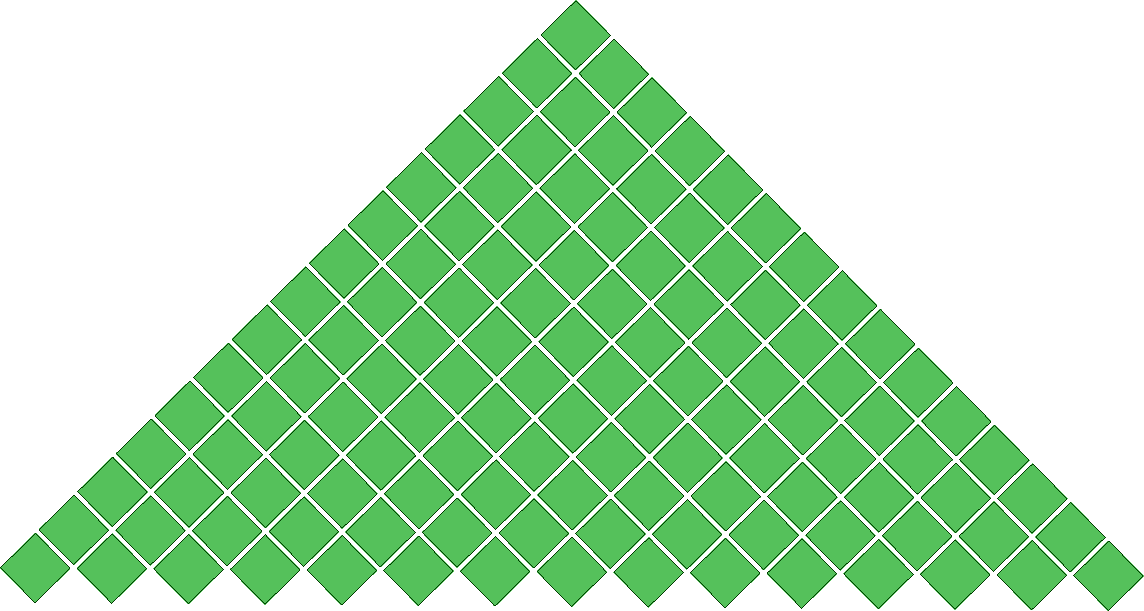
\includegraphics[width = 0.5\linewidth]{pic/mv008.pdf}}_{\text{$\omega = \omega_{1}\omega_{2} \dots \omega_{15} $}}
        \]
    \end{overprint}
    
\end{frame}

\begin{frame}[fragile] \frametitle{Application for the String-Searching Problem}

    \begin{itemize}
      \item \textbf{Problem:} for input string of length $n = 2^p - 1$ find all substrings of length \textit{m} which belong to $L_G(s)$
      \item \textbf{Valiant's algorithm:} it is necessary to calculate at least 2 triangle submatrices of size $\frac{n}{2}$ \\ 
      $\mathcal{O}(|G|BMM(2^{p - 1})(p - 2))$
    \end{itemize}

    \centering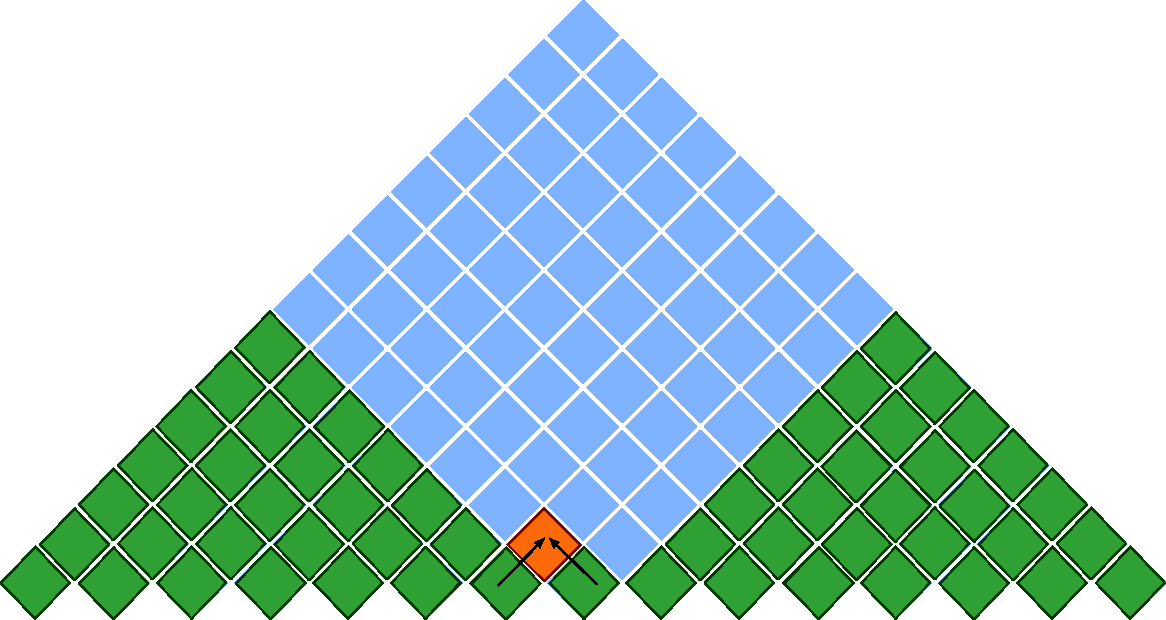
\includegraphics[width = 0.5\linewidth]{pic/valsubstring3.pdf}


    \pause
    \begin{itemize}
      \item  \textbf{Modification:} it is necessary to compute layers with submatrices of size not greater than $2^r$, where $2^{r-2} < s \le 2^{r - 1}$ \\
      $\mathcal{O}(|G|2^{2(p - r) - 1}BMM(2^{r})(r - 1))$
  \end{itemize}

\end{frame}

\begin{frame}[fragile] \frametitle{Evaluation}
    \begin{itemize}
        \item Implementation
        \begin{itemize}
            \item CPU-based: M4RI library
            \item GPU-based: CUDA C
        \end{itemize}
        \item Grammars
        \begin{itemize}
            \item $D_2$:
            \vspace{-12pt}
            \begin{figure}[t]
            %\subfloat{%
            \begin{minipage}{0.4\textwidth}
            \footnotesize
            \begin{alltt}
s: s s | ( s ) | [ s ] | \(\varepsilon \)
            \end{alltt}
            \end{minipage}
             % }
            \end{figure}

            \item \textit{BIO}:
            \vspace{-12pt}
            \begin{figure}[t]
            %\subfloat{%
            \begin{minipage}{0.4\textwidth}
            \footnotesize
            \begin{alltt}
s: stem<s0>
any_str: any_smb*[2..10]
s0: any_str | any_str stem<s0> s0
any_smb: A | T | C | G
stem1<s1>: A s1 T | G s1 C | T s1 A | C s1 G 
stem2<s1>: stem1<stem1<s1>>
stem<s1>:  
      A stem<s1> T 
    | T stem<s1> A 
    | C stem<s1> G 
    | G stem<s1> C 
    | stem1<stem2<s1>>              
            \end{alltt}
            \end{minipage}
             % }
            \end{figure}

        \end{itemize}
        
    \end{itemize}

\end{frame}
\begin{frame}{Data preprocessing}

    \begin{itemize}
        \item Example: n = 15, m = 6
    \end{itemize}

        $$
        \underbrace{
        \texttt{\color{blue}{AAGCTT}\color{white}{G}\color{blue}{AAGCTT}\color{white}{G}\color{blue}{AAGCTT}\color{white}{G}}
        }_{\text{len = 12}}
        $$
    \pause
        $$
        \underbrace{
        \texttt{\color{blue}{AAGCTT}\color{red}{G}\color{blue}{AAGCTT}\color{red}{G}\color{blue}{AAGCTT}\color{red}{G}}
        }_{\text{len = 15}}
        $$

\end{frame}

\begin{frame}{Results: Comparative Analysis}

%\\~

%    \begin{table*}
 %   \label{tbl1}
    \begin{center}
    \resizebox{\columnwidth}{!}{%
    \begin{tabular}{|| c||c|c|c|c || c|c|c|c ||} 
    \hline
    \multirow{3}{*}{n} & \multicolumn{8}{c||}{Time (sec)} \\
    & \multicolumn{4}{c||}{Grammar $D_2$} & \multicolumn{4}{c||}{Grammar $BIO$} \\
    & valCPU & modCPU & valGPU & modGPU & valCPU & modCPU & valGPU & modGPU   \\
    \hline
    127 & 0.08 & 0.08 & 0.20 & 0.10 & 1.35 & 1.34 & 0.19 & 0.10 \\
    255 & 0.28 & 0.30 & 0.52 & 0.13 & 5.40 & 5.50 & 0.53 & 0.14  \\
    511 & 1.21 & 1.18 & 1.90 & 0.25 & 21.97 & 22.35 & 1.99 & 0.26   \\
    1023 & 4.90 & 4.78 & 7.88 & 0.54 & 88.70 & 90.32 & 7.89 & 0.60  \\
    2047 & 19.61 & 19.38 & 33.50 & 1.50 & 363.32 & 374.20 & 34.01 & 1.70  \\
    4095 & 78.36 & 78.28 & 140.47 & 4.45 & 1467.68 & 1480.59 & 141.10 & 5.47 \\
    8191 & 315.67 & 315.08 & - & 13.65 & - & - & - & 18.04 \\
    \hline
    \end{tabular}
}
\end{center}

\onslide<2>{\tikz[overlay,remember picture]{\draw[fill=red, fill opacity=0.15] ($(1.04,0.45)$) rectangle ($ (3.7,3)$);}}
\onslide<2>{\tikz[overlay,remember picture]{\draw[fill=red, fill opacity=0.15] ($(6.34,0.45)$) rectangle ($ (9,3)$);}}
\onslide<3>{\tikz[overlay,remember picture]{\draw[fill=red, fill opacity=0.15] ($(3.5,0.45)$) rectangle ($ (6.16,3)$);}}
\onslide<3>{\tikz[overlay,remember picture]{\draw[fill=red, fill opacity=0.15] ($(8.8,0.45)$) rectangle ($ (11.5,3)$);}}
   
 %   \end{table*}
\end{frame}



\begin{frame}
\frametitle{Results: String-searching Problem}
    
 %   \begin{table*}
    
    \begin{center}
 %   \label{tbl3}
        \begin{tabular}{ ||c||c||c|c||c|c|| } 
        \hline
        \multirow{2}{*}{m}& \multirow{2}{*}{n} & \multicolumn{4}{c||}{Time (sec)}\\
        & & valCPU & modCPU & valGPU & modGPU \\
        \hline
        \multirow{4}{*}{250} & 1023 & 4.90 & 3.00 & 7.88 & 0.24 \\ 
        & 2047 & 19.61 & 6.65 & 33.50 & 0.26\\ 
        & 4095 & 78.36 & 13.83 & 140.47 & 0.32\\ 
        & 8191 & 315.67 & 28.90 & - & 0.46\\ 
        \hline
        \multirow{3}{*}{510} & 2047 & 19.61 & 12.18 & 33.50 & 0.58\\
        & 4095 & 78.36 & 26.58 & 140.47 & 0.65\\
        & 8191 & 315.67 & 56.70 & -  & 0.88\\ 
        \hline
        \multirow{2}{*}{1020} & 4095 & 78.36 & 48.31 & 140.47 & 1.59 \\
        & 8191 & 315.67 & 108.38 & - & 1.95\\ 
        \hline
        2040 & 8191 & 315.67 & 197.32 & - & 5.10\\ 
        \hline
        \end{tabular}
    \end{center}
    
  %  \end{table*}

\end{frame}


\begin{frame}[fragile] \frametitle{Conclusion}
    \begin{itemize}
        \item The modification of Valiant's algorithm was proposed
        \begin{itemize}
            \item Layered submatrices processing
            \item Effective utilization of parallel techniques and GPGPU
        \end{itemize}
        \item The modification is applicable to the string-searching problem
    \end{itemize}
\end{frame}

\begin{frame}[fragile] \frametitle{Future Research}
    \begin{itemize}
        \item Improvement of the existing implementation 
        \item Evaluation on real-world data
        \item Extension for more expressive classes of formal languages \\ (conjunctive,  Boolean)
    \end{itemize}
\end{frame}


\begin{frame}
\frametitle{Contact Information}
\begin{itemize}
  \item Semyon Grigorev: \href{mailto:semyon.grigorev@jetbrains.com}{semyon.grigorev@jetbrains.com}
  \item Yuliya Susanina: \href{mailto:jsusanina@gmail.com}{jsusanina@gmail.com}
  \item Anna Yaveyn: \href{mailto:anya.ayveyn@yandex.ru}{anya.ayveyn@yandex.ru}
\end{itemize}
\vspace{0.1cm}
\center{\huge{Thanks!}}
\end{frame}
\end{document}